\documentclass[11pt]{article}
\usepackage{titlesec}

\setcounter{secnumdepth}{4}

\parindent 0px % no automatic indentation

\usepackage{amsmath,amssymb,amstext,amsthm,amsfonts}
\usepackage{float}
\usepackage[shortlabels]{enumitem}
\usepackage[a4paper,lmargin={2cm},rmargin={2cm},tmargin={2.5cm},bmargin = {2.5cm},headheight = {4cm}]{geometry}

\usepackage[utf8]{inputenc}
\usepackage[T1]{fontenc}
%\usepackage[ngerman]{babel}
\usepackage{lmodern}
\usepackage{color}
\usepackage{xcolor}
\usepackage{colortbl}
\usepackage{graphicx}
\usepackage{listings}
\usepackage{xspace}
\usepackage{empheq}
\usepackage{mdframed}
\usepackage{changepage}
%\usepackage{hanging}
\usepackage{romanbar}
\usepackage{mathtools}
\usepackage[hidelinks]{hyperref}
\usepackage{empheq}
\usepackage{listings}
\usepackage{color}

\definecolor{codegreen}{rgb}{0,0.6,0}
\definecolor{codegray}{rgb}{0.5,0.5,0.5}
\definecolor{codepurple}{rgb}{0.58,0,0.82}
\definecolor{backcolour}{rgb}{0.95,0.95,0.92}

\lstset{language=R,
    basicstyle=\ttfamily\small,
    commentstyle=\color{codegreen},
    keywordstyle=\color{blue},
    numberstyle=\tiny\color{codegray},
    stringstyle=\color{codepurple},
    backgroundcolor=\color{backcolour},
    breaklines=true,
    captionpos=b,
    keepspaces=true,
    numbers=left,
    numbersep=5pt,
    showspaces=false,
    showstringspaces=false,
    showtabs=false,
    tabsize=2,
    frame=single
}

\usepackage[headsepline]{scrlayer-scrpage} 
\pagestyle{scrheadings} 
\usepackage{titling}
\usepackage{cancel}

\pagestyle{plain}

% MACROS
\newcommand{\ind}{\perp\!\!\!\!\perp} 

\title{Time Series Analysis Lecture Notes}

\author{Michael Sigg}
\date{\today}

\ohead{\theauthor}
\ihead{Time Series Analysis, Spring 24}



\begin{document}
\maketitle
\begin{center}
    Based on the course materials for the course Time Series Analysis FS24 by Prof. Damian Kozbur and TA Philipp Zhang, and the text book "The Analysis of Time Series: An Introduction with R" by Chris Chatfield and Haipeng Xing.
\end{center}
\tableofcontents

\newpage

\section{Introduction}



\subsection{Definition of Time Series}

A \textbf{Time Series} is a collection of data observations made sequentially over time.\\

\textbf{Examples of Time Series (from various scientific fields):}
\begin{itemize}
    \item \textbf{Economics}: Examples include unemployment rates, Gross National Product (GNP), gold prices, and exchange rates over time.
    \item \textbf{Finance}: Examples include stock returns and other financial metrics.
    \item \textbf{Geology}: Examples include temperature records, rainfall amounts, snow mass, and similar environmental measures.
    \item And many other fields.
\end{itemize}

\subsection{Types of Time Series (Terminology):}
\begin{enumerate}
    \item \textbf{Continuous Time Series}: These are observed at every point in time.
    \begin{itemize}
        \item Examples: humidity measurements, etc.
    \end{itemize}
    \item \textbf{Discrete Time Series}: These are observed at specific intervals.
    \begin{itemize}
        \item Examples: daily stock returns, quarterly unemployment figures, yearly avalanche deaths.
    \end{itemize}
\end{enumerate}

\subsection{Objectives in Time Series Analysis:}
\begin{enumerate}
    \item \textbf{Description}
    \begin{itemize}
        \item Begin with a time plot, where time is on the x-axis and the observed series value is on the y-axis.
        \item Look for features such as trends, seasonal variations, cyclical variations, regime shifts, and outliers.
    \end{itemize}
    \item \textbf{Explanation}
    \begin{itemize}
        \item More applicable to multivariate time series.
        \item For example, one might examine the relationship between unemployment and GDP.
        \item Methods to explain one time series using another include linear regression, nonlinear regression, and linear systems analysis.
    \end{itemize}
    \item \textbf{Prediction}
    \begin{itemize}
        \item Given a time series with values observed up to the present, predict the most likely future values.
        \item Examples: weather forecasting, GDP forecasting.
    \end{itemize}
    \item \textbf{Control}
    \begin{itemize}
        \item In many applications, it is possible to intervene and change the course of a time series.
    \end{itemize}
    \item \textbf{Statistical Inference}
    \begin{itemize}
        \item Involves conducting hypothesis tests or creating confidence intervals about parameters or properties of a time series.
        \item For example, determining if there is statistical evidence to conclude that a given time series contains a linear (non-zero) trend.
    \end{itemize}
\end{enumerate}


\section{Simple Descriptive Techniques}
In a introductory statistics class, one would calculate statistics like \textbf{sample mean} or \textbf{sample standard deviation} from data $x_i$ where $i$ indexes observations $i=1,...,n$ 
\begin{align*}
    \bar{x}&=\frac{1}{n}\sum_{i=1}^n x_i \\
    \hat{\sigma}&=\sqrt{\frac{1}{n}\sum_{i=1}^n (x_i - \bar{x})^2}
\end{align*}
However, in time series analysis, it is essential to describe \underline{types of variation}:
\begin{itemize}
    \item Seasonal variation
    \item Cyclical variation
    \item Trend
    \item Size of other irregular fluctuations
\end{itemize}

\bigskip
\underline{Trend}: 
\begin{itemize}
    \item[] Suppose data is denoted $x_1,...,x_t,...,x_T$ where:
    \begin{itemize}[label=\textbullet]
        \item $T$ is the length of the time series
        \item $t$ indexes time
        \item $x$ is a general variable to denote values
        \item $x_t$ is a value at time $t$
    \end{itemize}
\end{itemize}
$X_t = \alpha + \beta t + \varepsilon_t$, where $\varepsilon_t$ are irregular and "no trend" (later defined Stationarity) then $X_t$ has a linear trend with slope $\beta$ \\

\subsubsection{Basic Notation}

A time series is denoted $\{X_t\}_{t=1}^T$
\begin{itemize}
    \item $x$ is the variable observed
    \item $x_t$ is the value at time $t$
    \item $T$ is the length of the time series
    \item $X_t$ is a sequence of random variables $\Rightarrow$ Calculating mean or variance of $X_t$ is possible
\end{itemize}

\subsubsection{Breaking up a time series into components}
There are several types of components you might try to decompose a time series into
\begin{itemize}
    \item Deterministic Trend
    \item Seasonal or Cyclical variation
    \item Stationary component
\end{itemize}

\subsection{Formal Definition of Stationary Time Series}

\begin{mdframed}
A time series $\{X_t\}$ is \textbf{strictly stationary} if for any positive integer $k$ and $n$-tuple of positive integers $(t_1,t_2,...,t_n)$, the joint distribution function of $(X_t, X_{t_2},...,X_{t_n})$ equals the joint distribution function of $(X_{t+k}, X_{t_2+k}, ..., X_{t_n+k})$
\end{mdframed}


Intuitively, the time series "looks the same" in terms of its randomness at all points in time.\\

\textbf{Example:}\\

Let 
\[\Tilde{x}_t = 
\begin{cases} 
0 & \text{if day t's coin flip is heads}, \\
1 & \text{if day t's coin flip is tails}.
\end{cases}
\]
This is stationary.\\

Let

\[x_t = 
\begin{cases} 
0 & \text{if day t's coin flip is heads}, \\
1 & \text{if day t's coin flip is tails}. \\
\end{cases}
\]
except: \quad every time there are 3 heads in a row, do not toss a coin, but make the next point tails. If $\Tilde{x}_{t-3}=\Tilde{x}_{t-2}=\Tilde{x}_{t-1}=$ heads then assign $\Tilde{x}_t=$ tails.\\

\textbf{Properties}:
\begin{itemize}
    \item If $X_t$ and $Y_t$ are time series and they are independent from each other and $X_t$, $Y_t$ are stationary, then $X_t + Y_t$ is stationary
    \item If $X_t$ is stationary, then $X_t - X_{t-1}$ is stationary
\end{itemize}


\subsection{Trends in Time Series}

Trend refers to slow changes in the mean of a time series $X_t$. The simplest example of a time series with a trend is one of the form:\[
X_t = \alpha = \beta t + \varepsilon_t
\]
where \begin{itemize}
    \item $\alpha$ and $\beta$ are real numbers
    \item $\varepsilon$ is stationary \underline{and} mean zero.
\end{itemize}
Sometimes, write $\mu_t = \alpha + \beta t$ and assume $\mathbb{E}[\varepsilon_t]=0$. Call $\mu_t$ the mean of the time series. \\

Because
\begin{align*}
    \mathbb{E}[X_t] &= \mathbb{E}[\alpha + \beta t + \varepsilon_t] \\
    &= \mathbb{E}[\alpha + \beta t] + \mathbb{E}[\varepsilon_t] \\
    &= \alpha + \beta t + 0\\
    &= \mu_t
\end{align*}

\textbf{More general classes of trends:}
\begin{itemize}
    \item \textbf{Polynomial}: 
    \[X_t=\alpha+\beta t +\gamma t^2 + \nabla t^3 + \varepsilon_t\]
    \item \textbf{Geompertz trend}:
    \[X_t = \alpha exp(b\ exp(-ct)) + \varepsilon_t \quad c>0\]
    \item \textbf{Exponential}:
    \[X_t =a\ exp(bt) + \varepsilon_t\]
\end{itemize}
Models of Global trend: A small number of parameters captures information about the trend at all points in time.

\subsubsection{Estimating and Extracting Global Trends}

\textbf{Example: \quad Least Squares}

For a linear trend: \[X_t=\alpha + \beta t + \varepsilon_t\]

Estimate: \[(\hat{\alpha}, \hat{\beta})=\underset{a,b}{min} \frac{1}{T} \sum_{t=1}^T (X_t-a-bt)^2\]


$X_t =$ Trend$(X_t) + $ res$(X_t)$
\begin{itemize}
    \item res$(X_t)=\hat{\varepsilon}_t=X_t-\hat{\alpha} -\hat{\beta}t $
    \item Trend$(X_t)=X_t-$ res$(X_t)$
    \item Both are estimates. If $\varepsilon_t$ is stationary and $T$ large enough, then $\hat{\alpha}+\hat{\beta}t \approx \alpha+\beta t$ with high probability
\end{itemize}

\begin{figure}[H]
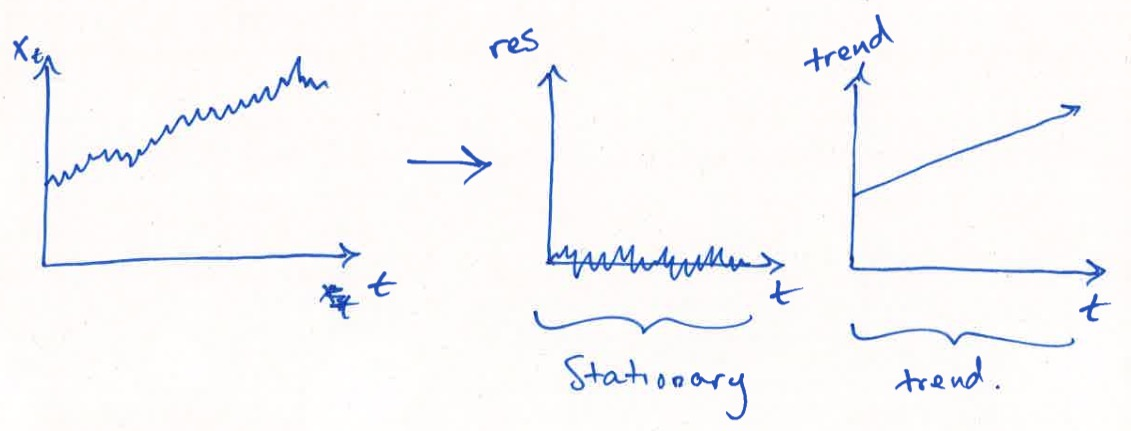
\includegraphics[scale=0.3]{images/Screenshot 2024-03-29 at 16.08.14.jpg}
\centering
\end{figure}

\subsubsection{Local Trend Extraction}

\textbf{\underline{Linear filtering}}: Transform $X_t$ into $Y_t$ according to \[Y_t = \sum_{r=-q}^S a_rX_{t+r}\] where $\{a_r\}$ is a set of weights. This operation is often called a moving average.\\

\textbf{Notation}: $Y_t=SM(X-t)$ \quad Sm="smoothed" \\

\textbf{Examples of Weight Schemes:}
\begin{itemize}
    \item Spencer's 15-point MA (moving average) with $q=7$:
    \[\{a_r\}=\frac{1}{320}(-3,-6,-5,3,27,46,67,74,67,...)\]
    \item Simple MA:
    \[a_r=\frac{1}{2q+1} \text{ for } r=-q,-q+1,...,q\]
\end{itemize}


\begin{figure}[H]
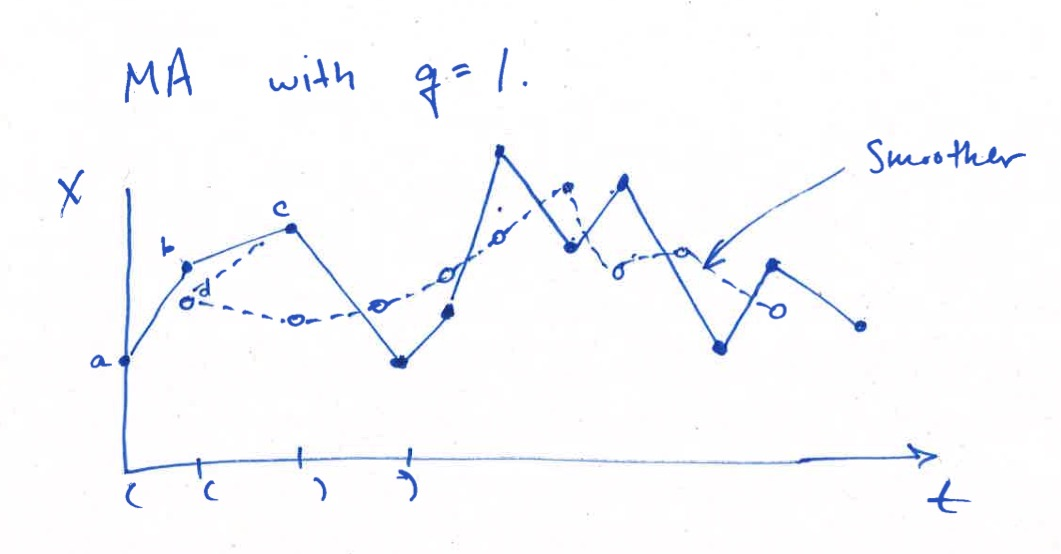
\includegraphics[scale=0.3]{images/Screenshot 2024-03-30 at 14.22.35.jpg}
\centering
\end{figure}


Again, like in Global trend extraction, for any linear filter, can calculate.
\[
\boxed{\text{res}(X_t)=X_t-\text{ Sm}(X_t)}
\]

\textbf{\underline{End effect problem}}: If observed $ \{X_t\}_{t=1}^T $ cannot smooth forward at $X_T$. With simple MA with $q=1$, $Sm(X_t)=\frac{1}{3}(X_{t-1}+X_t+X_{t+1})$. Cannot calculate $Sm(X_T)$ as $X_{T+1}$ is unknown. \\

Can use asymmetric filters:
\[Sm(X_t)=\sum_{r=-q}^0 a_r X_t\]
$\Rightarrow X_{t+1}$ never affects $Sm(X_t)$
\begin{itemize}
    \item Exponential Smoothing $Sm(X_t)=\sum_{j=0}^\infty a(1-a)^j x_{t-j}$
    \item First Difference average $Sm(X_t)=\frac{1}{2}(X_t+X_{t-1}$
\end{itemize}


\textbf{\underline{Differencing}}:
\begin{itemize}
    \item \textbf{First Order Differencing}: $Y_t =X_t-X_{t-1} = \nabla X_t$
    \item \textbf{Second Order Differencing}: $Z_t=\nabla Y_t= (X_t-X_{t-1})-(X_{t-1}-X_{t-2})=X_t-2X_{t-1}+X_{t-2}=\nabla^2X_t$
\end{itemize}

\textbf{\underline{Kernel Smoothing}}\\

Any type of smoothing where weights are specified by a Kernel function. 
\[Sm(X_t)=\sum_{t'=1}^T w_t(t'), \quad w_t(t')= \frac{K\left(\frac{t-t'}{b} \right)}{\sum_{t''=1}^T K\left( \frac{t-t''}{b}\right)}\]

\begin{itemize}
    \item "Kernel function" $K$. \quad Example: $K(\cdot)=e^{\frac{-(\cdot)^2}{2}}$
    \item "Bandwidth $b$" number 
\end{itemize}

\textbf{\underline{Sequential filtering (Convolution)}}

\bigskip

\begin{itemize}
    \item First, filter $\{X_t\}$ with weights $\{a_r\}$ to obtain $\{y_t\}$
    \item Then, filter $\{y_t\}$ with weights $\{b_j\}$ to obtain $\{z_t\}$
    \item To get the 'combined' weights $\{c_k\}$:
        \[
        z_t=\sum_j b_j y_{t+j}=\sum_jb_j \sum_r a_r x_{t+j+r} = \sum_k c_k X_{t+k}, \quad \text{ where } c_k=\sum_r a_r b_{k-r}
        \]
\end{itemize}

\subsubsection{Detrending a Time Series}

\begin{figure}[H]
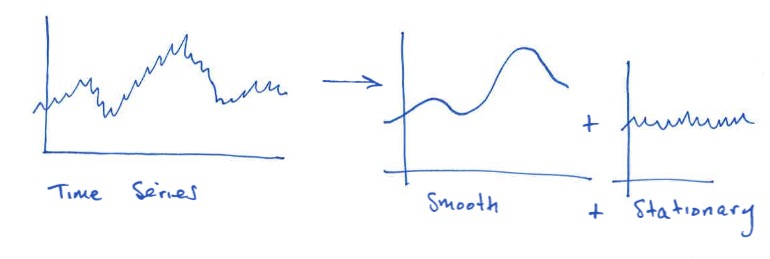
\includegraphics[scale=0.4]{images/Screenshot 2024-03-30 at 15.07.16.jpg}
\centering
\end{figure}

Global approach: Use a parametric functional form, e.g., $X_t=\beta t+\varepsilon_t$, $\beta$ estimated via least squares. \\

Local approach: Smoothing, $Y_t=Sm(X_t)=\sum_r a_r X_{t-r}$ \\

Detrending seasonality trends with local smoothing, e.g., the number of influenza cases recorded, is seasonal because there is a predictable peak in winter.\\

\textbf{Standard for Seasonality:}
\begin{align*}
    Y_t=Sm(X_t)&=\frac{0.5 X_{t-6} + X_{t-5}+...+X_{t+5} + 0.5 X_{t+6}}{12}\\
    Res(X_t)&=X_t-Sm(X_t) \quad \text{$\Rightarrow$ num. of surprise cases}
\end{align*}

Other procedures are available too, used by e.g., US Census Bureau:
\begin{itemize}
    \item X12 ARIMA
    \item SEATS-TRAMO
    \item X13 ARIMA-SEATS
\end{itemize}

\subsection{Autocorrelation and the Correlogram}

\textbf{Goal}: Come up with a method for measuring dependence between observations across time.\\

Remember the definition of sample correlation of two random variables $\Romanbar{X}$ and $\Romanbar{Y}$ with data $(X_1,Y_1), ..., (X_T,Y_T)$
\begin{align*}
    r&=\frac{\sum_{t=1}^T (X_t-\bar{X})(Y_t-\bar{Y})}{\sqrt{\sum_{t=1}^T (X_t-\bar{X})^2 \times \sum_{t=1}^T (Y_t-\bar{Y})^2}} \\
    \bar{X}&= \frac{1}{T} \sum_{t=1}^T X_t &&= \text{average}(\Romanbar{X}) \\
    \bar{Y} &= \frac{1}{T} \sum_{t=1}^T Y_t &&= \text{average}(\Romanbar{Y})
\end{align*}
If $X_t=Y_t$? Then $r=1$\\




Apply correlation idea to lags of time series
\begin{itemize}
    \item For example, let $(X_t, Y_t)=(X_t, X_{t-1})$
    \item Warning: this only measures "linear dependence"
\end{itemize}


Define:
\begin{align*}
        r&=\frac{\sum_{t=1}^{T-1} (X_t-\bar{X}_{(1)})(X_{t+1}-\bar{X}_{(2)})}{\sqrt{\sum_{t=1}^{T-1} (X_t-\bar{X}_{(1)})^2 \times \sum_{t=1}^{T-1} (X_{t+1}-\bar{X}_{(2)})^2}} \\
        \bar{X}_{(1)} &= \sum_{t=1}^{T-1} \frac{X_t}{T-1} \\
        \bar{X}_{(2)} &= \sum_{t=1}^{T-1} \frac{X_{t+1}}{T-1} 
\end{align*}

Most researchers use approximation $\bar{X}_{(1)} \approx \bar{X}_{(2)} \approx \bar{X} $ and terms in the denominator are approximately equal. This gives 
\[r_1=\frac{\sum_{t=1}^{T-1} (X_t-\bar{X})(X_{t+1}-\bar{X})}{\sum_{t=1}^{T} (X_t-\bar{X})^2}\]

Terminology for $_1$:
\begin{itemize}
    \item Sample autocorrelation of lag 1
    \item First order autocorrelation coefficient
    \item Usage of terminology is author dependent
\end{itemize}

For larger lags, let $k>0$ be an integer lag:
\[r_k=\frac{\sum_{t=1}^{T-k} (X_t-\bar{X})(X_{t+k}-\bar{X})}{\sum_{t=1}^{T} (X_t-\bar{X})^2}\]

\begin{itemize}
    \item $k$-th order autocorrelation coefficient
    \item Caution: Really only used for stationary time series
\end{itemize}

\textbf{Exc. 2.4 (Book)}: With a truly random process (under the assumption of a Gaussian white noise process) it is expected that the sample autocorrelation coefficient fall inside the C.I. that is given as: $\pm z\times \sqrt{\frac{1}{N}}$. (Note: in a random process it is normal to find some coefficient to fall just outside the C.I.)\\


\textbf{\underline{Correlogram}}: \\

A plot of autocorrelation coefficients.

\begin{itemize}
    \item Choose a number $M<T$. E.g., if $T=200$, $M=30$ might be used
\end{itemize}

\begin{lstlisting}[language=R]
# In R (status package)
acf(x)        #(uses M=10*log_10(T))
                #(Horizontal bounds at +- 2/\sqrt(T) )
\end{lstlisting}

Example:

\begin{figure}[H]
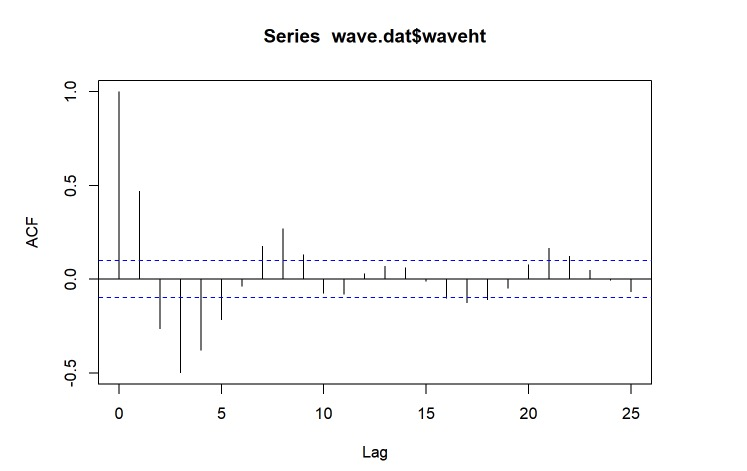
\includegraphics[scale=0.4]{images/Screenshot 2024-03-30 at 17.42.36.jpg}
\centering
\end{figure}


\subsection{Transformations}

In many cases, to reduce the unwanted effects of outliers, statistical routines can apply transformations to a time series.\\

Example:

\begin{figure}[H]
  \centering
  \begin{minipage}{0.49\textwidth}
    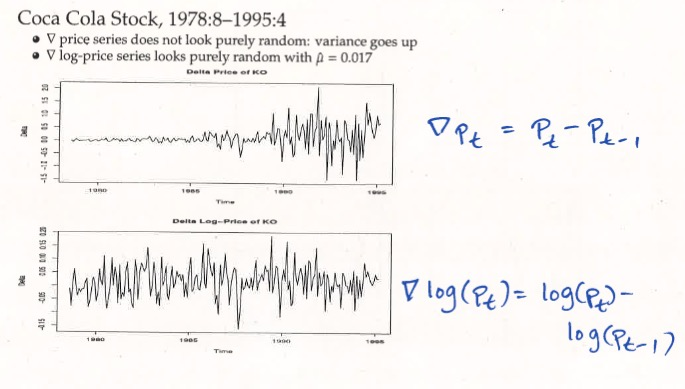
\includegraphics[height=5cm]{images/Screenshot 2024-03-30 at 17.45.04.jpg} % Left image
  \end{minipage}\hfill
  \begin{minipage}{0.49\textwidth}
    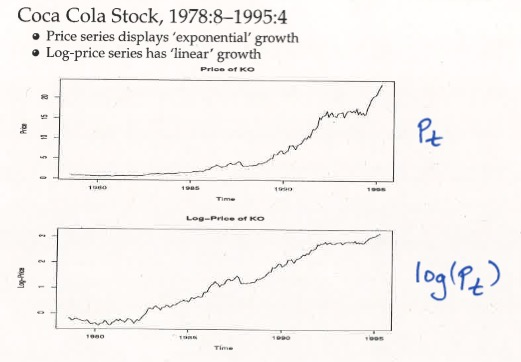
\includegraphics[height=5cm]{images/Screenshot 2024-03-30 at 17.46.58.jpg} % Right image
  \end{minipage}
\end{figure}





\section{Linear Time Series Models}
\textbf{Building block time series processes.}\\


The simplest time series is a independent and identically distributed (iid.) series: $X_t = \varepsilon_t$, where $\varepsilon_t$ are iid.\\

We can build a more complicated process assuming assuming access to $\varepsilon_t$:

\begin{align*}
    X_t&= \varepsilon_t + 0.9\varepsilon_{t-1} &&\text{(Moving Average)} \\
    X_t&= 0.9X_{t-1} + \varepsilon_t &&\text{(Autoregressive Process)} \\
    X_t&= \pm \sqrt{|-0.8X_{t-1} + \varepsilon_t|} &&\text{(Nonlinear Process)}
\end{align*}

\subsection{Definitions}

A \textbf{stochastic process} is a collection of random variables that are ordered (indexed) in time.

\begin{itemize}
    \item[]
    \begin{itemize}
        \item Note: they may be discrete or continuous
    \end{itemize}
    \item For each $t$ there is a random variable $\Romanbar{X}_t$, and the collection can simply be called $\Romanbar{X}$.
    \item Usually "realizations" of $\Romanbar{X}_t$ are labeled $X_t$
    \item[$\rightarrow$] You can think of $\Romanbar{X}$ as a multivariate random variable, where components are ordered
\end{itemize}

Let $\Romanbar{X}$ be a stochastic process.\\

$\Romanbar{X}$ is \textbf{\underline{strictly stationary}} if the distribution (joint) of $(\Romanbar{X}_t, \Romanbar{X}_{t_2}, ..., \Romanbar{X}_{t_k} $ is invariant to shifts. (Equal to distribution of $(\Romanbar{X}_{t_1+h}, \Romanbar{X}_{t_2+h}, ..., \Romanbar{X}_{t_k+h} $)\\

Strict stationarity is difficult to satisfy and verify. \\

$\Romanbar{X}$ is \textbf{\underline{mean stationary}} if the mean function $\mu_t = E[\Romanbar{X}_t]$ is constant and does not depend on $t$.\\


$\Romanbar{X}$ is \textbf{\underline{covariance stationary}} if:
\begin{itemize}
    \item The mean function $\mu_t=\mathbb{E}[\Romanbar{X}_t]$ is constant (doesn't depend on t)
    \item The variance function $\sigma^2_t=Var(\Romanbar{X}_t)$ is constant
    \item The autocovariance function $\gamma(t,s)=Cov(\Romanbar{X}_t,\Romanbar{X}_s)$ depends only on $t-s$
\end{itemize}

Let $\tau=t-s$ $\Rightarrow \gamma(\tau) = Cov(\Romanbar{X}_t, \Romanbar{X}_s)$ only makes sense if $Cov(\Romanbar{X}_t,\Romanbar{X}_s)=Cov(\Romanbar{X}_{t+1},\Romanbar{X}_{s+1})$, etc.\\

$\Romanbar{X}$ is \textbf{\underline{weakly stationary}} (also known as second-order stationarity) if it satisfies the conditions of both mean stationarity and covariance stationarity.

\subsection{The Random Walk}

\[\Romanbar{X}_t=\Romanbar{X}_{t-1}+\varepsilon_t, \quad  \varepsilon_t \text{ iid.}\]
Note: Random walk on integer lattice occurs when $\varepsilon_t \in \{-1,1\}$ 50/50 and sometimes $\Romanbar{X}_0=0$  \\

\textbf{Mean function}: (for the case $\Romanbar{X}_0=0$)
\begin{align*}
    \mu_t=\mathbb{E}[\Romanbar{X}_t] &= \mathbb{E}[\Romanbar{X}_{t-1} + \varepsilon_t]\\
    &=\mathbb{E}[\Romanbar{X}_{t-2}+\varepsilon_{t-1}+\varepsilon_t] \\
    & \vdots\\
    &=\mathbb{E}[\varepsilon_1+...+\varepsilon_t] \\
    &=t * \mathbb{E}[\varepsilon_1]
\end{align*}
\begin{itemize}
    \item If $\mathbb{E}[\varepsilon_1=0]$ (without drift), then $\mu_t=0$, which does not depend on $t$.
    \item If $\mathbb{E}[\varepsilon_t\neq 0]$, this is called a random walk with drift
\end{itemize}

\textbf{Variance function:}
\begin{align*}
    \sigma^2=var(\Romanbar{X}_t)&=var(\Romanbar{X}_{t-1} + \varepsilon_t)\\
    &=var(\Romanbar{X}_{t-2} + \varepsilon_{t-1} + \varepsilon_t) \\
    &\vdots \\
    &=var(\varepsilon_1+...+\varepsilon_t)\\
    &=var(\varepsilon_1)+...+var(\varepsilon_t)\\
    &=t * var(\varepsilon_t)
\end{align*}
$\sigma^2$ depends on $t$ if $Var(\varepsilon_1)\neq 0 \Rightarrow$ not covariance stationary \\

A popular simple model for stock prices is that $\log(price_t)$ is a random walk.

\subsection{The Backshift Operator $B$}

Let $\Romanbar{V}$ be a stochastic process. Then $B\Romanbar{V}$ is another stochastic process with \[(B\Romanbar{V})_t=\Romanbar{V}_{t-1}\]

\begin{itemize}
    \item More common notation: $B\Romanbar{V}_t=\Romanbar{V}_{t-1}$
    \item Also called "Lag" operator 
    \item $B^2\Romanbar{V}_t=B\Romanbar{V}_{t-1}=\Romanbar{V}_{t-2}$, \quad $B^k\Romanbar{V}_t=\Romanbar{V}_{t-k}$
    \begin{itemize}
        \item[] Note: Book uses $\nabla$ to be difference operator 
        \[ \nabla=1-B \text{ because: } \nabla V_t = V_t-V_{t-1}=V_t-BV_t=(1-B)V_t\]
    \end{itemize}
\end{itemize}

\textbf{Building a random walk with the backshift operator:}
\begin{align*}
    \Romanbar{X}_t&=\Romanbar{X}_{t-1}+\varepsilon_t\\
    \Rightarrow \Romanbar{X}_t-\Romanbar{X}_{t-1}=\varepsilon_t\\
    \Rightarrow(1-B)\Romanbar{X}_t=\varepsilon_t
\end{align*}

\textbf{Note:} "$1-B$" is not invertible; thus division by $1-B$ is not possible

\subsection{Moving Averages}

\begin{align*}
  \Romanbar{X}_t&=\sum_{i=0}^q \theta_i\varepsilon_{t-i} &&\text{is called a $q$-order moving average. Also called "$MA(q)$"} 
\end{align*}
\begin{align*}
  &= \underbrace{(\theta_0+\theta_1B+...+\theta_qB^q)}_{\text{polynomial in $B$ with coefficients $\theta_0...\theta_q$, real numbers usually}}\varepsilon_t
\end{align*}
\begin{align*}
  \Romanbar{X}_t&=p(B)\varepsilon_t &&\text{usually rescale $\varepsilon_t$ so that $\theta_0=1$}
\end{align*}

\textbf{Basic calculations}: Assume $\mathbb{E}[\varepsilon_t]=0$. Then: 
\begin{align*}
    \mu_t=\mathbb{E}[\Romanbar{X}_t]=\mathbb{E}[\sum_{i=0}^q \theta_i \varepsilon_{t-1}]=\sum_{i=0}^q \theta_i \mathbb{E}[\varepsilon_{t-1}]=0 \\
\sigma^2_t=var(\Romanbar{X}_t)=\sum_{i=0}^q \theta_i^2 var(\varepsilon_{t-1}) 
\end{align*}

\textbf{Invertibility of Moving Averages}
\begin{align*}
    \Romanbar{X}_t&= \sum_{i=0}^q \theta_i\varepsilon_{t-i}\\
    &=p(B)\varepsilon_t\\
\end{align*}
$p(B)$ is the "Lag polynomial" or "Backshift polynomial"\\

\textbf{Theorem}: $\varepsilon_t$ can be written as $\varepsilon_t=q(B)\Romanbar{X}_t$ for some (possibly infinite) lag polynomial $q(B)$ if all roots of $p$ (i.e., meaning complex solutions to $p(z)=0$) have $|z|>1$, equivalently lie outside the unit circle. \\

\textbf{Motivation}: The imposition of an invertibility condition ensures that there is a unique MA process for a given ac.f.

\textbf{Example:} In Random Walk:
\begin{align*}
    \Romanbar{X}_t&=\Romanbar{X}_{t-1}"\varepsilon_t\\
    \Rightarrow (1-B)\Romanbar{X}_t&=\varepsilon_t
\end{align*}
If $p(B) = 1-B$, then:
\begin{align*}
    p(B)\Romanbar{X}_t&=\varepsilon_t
\end{align*}

The roots of $p(B)$ thought of as a regular polynomial $p(z)$ are $p(z)=1-z$, which vanishes at $z=1$.
\begin{itemize}
    \item Called unit root because $|z|=1$
    \item Unit roots $\Rightarrow$ non-Stationarity
\end{itemize}
 Know random walk is not stationary:
\[\sigma^2_t=t \cdot var(\varepsilon_1)\]

\subsection{Autoregressive Process}

$\Romanbar{X}_t$ is an autoregressive process of order $p$ if:
\[\Romanbar{X}_t=\varphi_0+\varphi_1\Romanbar{X}_{t-1}+\varphi_2\Romanbar{X}_{t-2}+...+\varphi_p\Romanbar{X}_{t-p}+\varepsilon_t\]

This can be written as a Lag polynomial applied to $\Romanbar{X}$:
\begin{align*}
    q(B)\Romanbar{X}_t&=\varepsilon_t+\varphi_0\\
    q(B)&=1-\varphi_1\Romanbar{X}_{t-1}-...-\varphi_p\Romanbar{X}_{t-p}
\end{align*}

\begin{itemize}
    \item AR(1):
    \begin{align*}
        X_t&=\mu_t+\alpha_1 BX_t +\varepsilon_t\\
        &=\mu+\alpha X_{t-1}+\varepsilon_t
    \end{align*}
    \item AR(p): $X_t=\mu+\alpha_1 X_{t-1}+...+\alpha_pX_{t-p}+\varepsilon_t $
    \item[] Regression of $X$ on its own past
\end{itemize}

Any AR($p$) process:
\begin{itemize}
    \item Can be written as an MA($\infty$) process, but there are no easy formulas for the MA coefficients when $p\geq 2$
    \item Is, by definition, invertible.
\end{itemize}

The process is stationary if the roots of the equation \[
\phi(x)=1-\sum_{i=1}^p \alpha_i x^{i} = 0
\] (where $x$ is potentially complex) lie outside the unit circle.\\

To find the ac.f. in the stationary case, from $X_t=\sum_{i=1}^p \alpha_i X_{t-i}+Z_t$, where the $\alpha_i$ are constants, we get:\[\rho(k)=\sum_{i=1}^p \alpha_i\rho(k-i) \quad \forall k>0\]

This set of equations is called the \textbf{Yule-Walker equations}.\\

The set of Yule-Walker equations has the general solution \[
\rho(k) = \sum_{i=1}^p A_i\pi_i^{|k|}
\]
where the $\{\pi_i\}$ are the roots of the so-called auxiliary equation \[
y^p - \sum_{i=1}^p \alpha_i y^{p-i}=0
\]
The constants $\{A_i\}$ are chosen to satisfy the initial conditions:
\begin{itemize}
    \item $\rho(0)=1 \Rightarrow \sum A_i = 1 $
    \item The first ${p-1}$ Yule-Walker equations provide $(p-1)$ further restrictions on the $\{A_i\}$, using $\rho(0)=1$ and $\rho(k)=\rho(-k)$
\end{itemize}
Alternative (but equivalent) condition for stationarity:
\begin{itemize}
    \item The roots $\{\pi_i\}$ of the auxiliary equation all statisfy $|\pi_i|<1$
\end{itemize}


\subsection{ARMA(p,q)}

ARMA combines MA and AR processes:

\begin{itemize}
    \item ARMA(1,1): \[
    X_t = \overbrace{\mu}^{\mathclap{\text{Intercept parameter}}} + 
    \underbrace{\alpha X_{t-1}}_{\mathclap{\text{Autoregressive component}\phantom{ \quad \quad \quad \quad\quad \quad \quad}}} + 
    \overbrace{\varepsilon}^{\mathclap{\text{Shock}}} + 
    \underbrace{\beta \varepsilon_{t-1}}_{\mathclap{\text{Moving average component}}}
    \]
    \item ARMA(p,q): \[
    X_t=\mu+\alpha_1 X_{t-1} +...+\alpha_p X_{t-p}+ \varepsilon_t + \beta_1 \varepsilon_{t-1}+...+ \beta_q \varepsilon_{t-q}
    \]
    \begin{itemize}
        \item "Regression on own history and shock history"
        \item Example: \(X_t=\mu+\Phi(B)X_t+\varepsilon_t+\psi(B)\varepsilon_t \)
    \end{itemize}
\end{itemize}

The condition for \textbf{stationarity} is that the AR part $\phi(B)$ is stationary.\\
The condition for \textbf{invertibility} is that the MA part $\theta(B)$ is invertible.

\subsection{ARIMA(p,d,q)}

ARIMA Model for \(\nabla X_t=X_t-X_{t-1}\)
\begin{itemize}
    \item[] E.g., \( ARIMA(1,1,1)=\nabla X_t=\mu +\alpha \nabla X_{t-1} + \varepsilon_t + \beta \varepsilon_{t-1} \)
    \item $ARIMA(p,d,q)$ \quad $d$: number of times $\nabla$ is applied
\end{itemize}

\subsection{SARIMA}

\[SARIMA(p,d,q) x (P,D,Q)_s\]

In practice, many time series contain a seasonal periodic component, which repeats every $s$ observations. \\

A general multiplicative seasonal ARIMA model (SARIMA) is defined as: \[
\phi_p(B) \Phi_P(B^s)W_t = \theta_q(B)\Theta_Q(B^s)Z_t 
\]
where $B$ denotes the backwards shift operator, $\phi_p, \Phi_P, \theta_q, \Theta_Q$ are polynomials of order $p,P,q,Q$, respectively, $Z_t$ denotes a purely random process and \[ W_t=\nabla^d \nabla^D_s X_t \] denotes the differenced series.

\textbf{Example}: $ARIMA(1,0,0)\times(0,1,1)_12$
\begin{align*}
    \phi_1(B) \cancel{\Phi_0(B^{12})} \cancel{\nabla^0} \nabla^1_{12} X_t = \cancel{\theta_0(B)}\Theta_1(B^{12})Z_t \\
    (1-\phi_1 B)(X_t-X_{t-12})=(1+\Theta B^{12})Z_t \\
    X_t = X_{t-12} + \phi_1(X_{t-1}-X_{t-13}) + Z_t + \Theta_1 Z_{t-12}
\end{align*}

\subsection{Exercise 3}
\begin{itemize}
    \item Deriving ac.f. 
    \begin{enumerate}
        \item[] $\rho(k)=\frac{Cov(X_\cdot, X_{c\cdot + k})}{Var(X_\cdot)} $
        \item Calculate $\mathbb{E}[X_t]$
        \item Calculate $\mathbb{E}[X_t X_{t+k}] = Cov$
        \item Calculate $Var(X_t)$
    \end{enumerate}
    \item Assessing Stationarity:
    \begin{itemize}
        \item Look at the characteristic polynomial of an AR process, if all roots lie outside the unit circle ($|root|>1$) the model is stationary.
    \end{itemize}
    \item Assessing Invertibility:
    \begin{itemize}
        \item Look at the characteristic polynomial of an MA process, roots again must lie outside the unit circle
    \end{itemize}
    \item Reminder: quadratic formula:
    \begin{align*}
        \text{If } ax^2 +bx+c=0 \\
        x=\frac{-b \pm \sqrt{b^2-4ac}}{2a}
    \end{align*}
\end{itemize}

\section{Model Fitting \& Selection}
\subsection{Fitting}

Given an observed time series, estimate which model best approximates its dynammics:\\
\quad Choose from $\overbrace{AR(p),MA(q),ARMA(p,q),...}^\text{Model Selection}$ and estimate parameters (e.g., $\underbrace{\alpha_1,...\alpha_p, \beta_1,...,\beta_q}_\text{estimation}$).

\bigskip
\textbf{\underline{Inference}}: \quad Draw confidence intervals for parameters estimates

\textit{Note}: Inference for the mean of a stationary time series:

Let $X_t$ be a stationary time series. That means $E[X_t]=E[X_{t+1}]=E[X_{t+2}]=...=\mu $. So $\mu$ is "population unconditional mean". Let $\gamma_k$ be the $k^{-th}$-order population autocovariance
\[
\gamma_k=Cov(X_t,_{t-k})
\]
Problem: Confidence interval for $\mu$ given $X_1,...,X_T$

\begin{figure}[h]
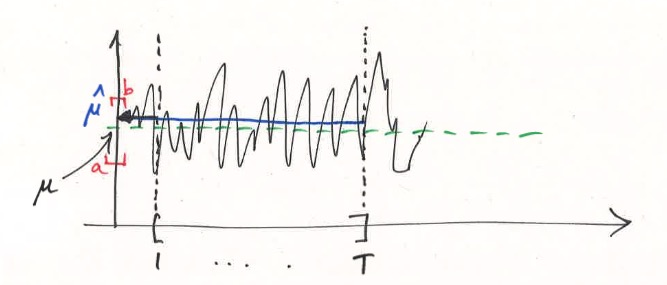
\includegraphics[scale=0.4]{images/Screenshot 2024-03-31 at 16.34.09.jpg}
\centering
\end{figure}

Regular stats confidence interval (margin of error measure): $\hat{\mu}=\frac{1}{T}\sum_{t=1}^T X_t=\bar{X}_T$\\

Want: C.I [a,b] s.t. $Pr(\mu$ in [a,b]$) \geq 95\%$

\bigskip

\underline{Strategy}:

\begin{itemize}
    \item Calculate $var(\hat{\mu})=var(\bar{X}_T) $
    \item By Central Limit Theorem, $\Rightarrow \hat{\mu} \approx$ Gaussian
    \item use 95\% quantiles of Gaussian with variance $var(\hat{\mu})$
    \item Produce a formula that can be coded and given to computer
\end{itemize}
Fact: If $\hat{\gamma}_k$ are sample analogues: do not use all of them for the sum because \begin{align*}
    \hat{var}(\hat{\mu}) &= \frac{1}{T}\sum_{t=1}^T var(X_t) + \frac{1}{T^2} \sum_{t\neq t} Cov(X_t, X_s) \\
    &= \frac{1}{T} T \hat{\gamma}_0 + \frac{1}{T^2} \sum_{s\neq t} \hat{\gamma}_k\\
    &= \hat{\gamma}_0 + \frac{1}{T^2} \sum_{k=1}^T \hat{\gamma}_k \cdot (T-k)
    &\text{vanishes $(=0)$ degrees of freedom problem}
\end{align*}
So instead, truncate at a given lag $h$. $l<<h<<T$ \quad Say \( \lfloor \sqrt{T} \rfloor \) or \( \lfloor log T \rfloor \)
\[
\hat{var}(\hat{\mu})=\frac{\hat{\gamma}_0}{1} + \frac{1}{T^2}\sum_{k=1}^h \hat{\gamma}_k (T-k)
\]
Then C.I $[a,b]=\hat{\mu} \pm 1.96 \sqrt{\hat{var}(\hat{\mu})} $
Sometimes called $\underbrace{\text{"HAC"}}_\text{heteroskedasticity, autocorrelation consistent}$ estimator

\begin{align*}
    var(\hat{\mu})&=var(\frac{1}{T}\sum_{t=1}^T X_t) \leftarrow \text{ difficult to expand if $Cov(X_t, X_s)\neq 0$}\\
    &=\frac{1}{T^2} \sum_{t=1}^T var(X_t) + \frac{1}{T^2} \sum_{s\neq t} Cov(X_t,X_s)\\
\end{align*}

usually with iid. data: would just estimate $\hat{var}(\hat{\mu})=\frac{1}{T}\sum_{t=1}^T(X_t-\hat{\mu})^2=\hat{\gamma}_0 $. Then form C.I.: $\hat{\mu}\pm 1.96 \times \hat{\gamma}_0^\frac{\sqrt{\hat{\gamma}_0}}{\sqrt{T}} $

\underline{In time series data}:
\begin{itemize}
    \item Can form $\hat{\gamma}_k$ for all $k$, and use it carefully
\end{itemize}


\subsection{PACF}

\underline{Partial Autocorrelation Function}, and choosing between $AR(p_1)$ and $AR(p_2)$ for 2 different Lags.

\textbf{\underline{Definition}}: \quad The function $PACF(k)$ is defined by the estimate $\pi_k$ in the least squares fit: \[
X_t=\nu +\pi_1 X_{t-1} +...+ \pi_k X_{t-k}
\]
In stats software packages, ---- bounds are drawn at $\pm \frac{2}{\sqrt{T}}$ like for auto correlation functions when properly normalized: do this with unit variance scaling of $X_t$ (means replace $X_t$ with $\frac{X_t}{var(X_t)}=\frac{X_t}{\sigma^2}$)(Software does this automatically)

\begin{itemize}
    \item The PACF essentially isolated the direct effect of lag $k$ on the correlation, removing the influence of intermediate lags.
    \item This helps identifying the order of AR terms in ARMA models: Significant spikes in the PACF at specific lags indicate potential AR components. A cut-off after lag $p$ in the PACF suggests an $AR(p)$ model might be appropriate
\end{itemize}

\subsection{Estimation}

Least squares estimation for $\varepsilon_t$ estimates. !- Least squares is Maximum Likelihood for $\varepsilon_t$ Gaussian \\

For general $ARMA(p,q)$ model:

$ARMA(1,0)$: \[
X_t=\mu+\alpha X_{t-1} + \varepsilon_t+\beta\varepsilon_{t-1}
\]
\begin{itemize}
    \item Assume $\beta=0$ to start easy
    \item[] Given candidate $\alpha, \mu$ call it $\alpha^{\textit{candidate}}, \mu^{\textit{cand.}}$ Form: \[\hat{\varepsilon}(\alpha^{\textit{cand.}},\mu^{\textit{cand.}}) = X_t -\mu^{\textit{cand.}} - \alpha^{\textit{cand.}}X_{t-1}
    \]
    \item[] Calculate: \[SS(\alpha^{\textit{cand.}},\mu^{\textit{cand.}})=\sum_{t=2}^T \hat{\varepsilon}_t(\alpha^{\textit{cand.}},\mu^{\textit{cand.}} )^2 \]
    \item[] Take $\hat{\alpha}, \hat{\mu}$ to be minimizer of $SS(\alpha^{\textit{cand.}},\mu^{\textit{cand.}})$
\end{itemize}

Straight generalization to $MA(q)$ or $ARMA(p,q)$ etc. is \underline{not} straight forward.

\textbf{With MA}
\begin{itemize}
    \item $X_t=\mu+\varepsilon_t+\theta\varepsilon_{t-1}$ $\leftarrow$ Hard to do the instinctive thing, e.g.,
    \begin{itemize}
        \item[] $X_t-\mu-\varepsilon_t-\theta\varepsilon_{t-1}=0$
        \item[] $\underbrace{\varepsilon_t=X_t-\mu-\theta\varepsilon_{t-1}}_\text{Cannot square these and sum, because $\varepsilon_{t-1}$ is on inside.}$
        \begin{itemize}
            \item[] $\rightarrow$ Don't have an ex ante estimate $\hat{\varepsilon}_{t-1}$ \underline{unless} we approximate ("initialize") $\hat{\varepsilon}_0=0$
        \end{itemize}
    \end{itemize}
    \item For candidate $\mu^{\textit{cand.}}$, $\theta^{\textit{cand.}}$
    \begin{itemize}
        \item[]
        \begin{align*}
            \hat{\varepsilon}_1&=X_1-\mu^{\textit{cand.}}-\theta^{\textit{cand.}}\cdot \underbrace{\hat{\varepsilon}_0}_{=0}\\
            &=X_1-\mu^{\textit{cand.}}\\
        \end{align*}
        \item[]$\Rightarrow$ $\hat{\varepsilon}_1$ can be calculated now
        \begin{align*}
            \hat{\varepsilon}_2=X_2-\mu^{\textit{cand.}}-\theta^{\textit{cand.}} \cdot \hat{\varepsilon}_1
        \end{align*}
        \item[]$\Rightarrow$ $\hat{\varepsilon}_2$ can be calculated 
        \item[] etc.
    \end{itemize}
    \item[] Let $\hat{\mu}, \hat{\theta}$ $\underset{\mu^{\text{cand.}},\theta^{\text{cand.}}}{\text{minimize}}$ $\sum_{t=1}^T \hat{\varepsilon}_t^2$
    \begin{itemize}
        \item[] For finite order $MA(q)$, bias $\sim \frac{1}{T}$ is "small"
        \item[] ! This is smaller than $\frac{1}{\sqrt{T}}$, the statistical margin of error for $\hat{\mu}, \hat{\theta}$
    \end{itemize}
\end{itemize}

\textbf{General $ARMA(p,q)$ model:} \quad Least Squares Approach
\[
X_t=\mu+\alpha_1X_{t-1}+...+\alpha_p X_{t-p}+\varepsilon_t+\theta_1 \varepsilon_{t-1}+...+\theta_q\varepsilon_{t-q}
\]
\begin{itemize}
    \item Inititalize $\hat{\varepsilon}_0, \hat{\varepsilon}_{-1},...,\hat{\varepsilon}_{-q+1}=0 $
    \item[$\Rightarrow$] can calculate $\hat{\varepsilon}_1,\hat{\varepsilon}_2,...,\hat{\varepsilon}_T $ recursively, given candidate parameters
    \begin{itemize}
        \item Then minimize $\sum_{t=1}^T\hat{\varepsilon}_t^2 $
        \begin{itemize}
            \item[$\rightarrow$] $\hat{\mu},\hat{\alpha}_1,...,\hat{\alpha}_p, \hat{\theta}_1,...,\hat{\theta}_q $
        \end{itemize}
    \end{itemize}
    \item[] Can also minimize over $\hat{\varepsilon}_0$, computationally difficult 
\end{itemize}
\fbox{Maximum Likelihood Estimation} \quad (Alternative to Least Squares)
\begin{itemize}
    \item Native in Software
    \item Equivalent to Least Squares if $\varepsilon_t \sim N(0,\sigma^2)$, (i.e., $\varepsilon_t$ are Gaussian)
    \item Flexible enough that it can allow non-Gaussian $\varepsilon_t$ by appropriate adjustment to Likelihood
\end{itemize}

\subsection{Model Selection}

\begin{itemize}
    \item[] For $ARMA(p,q)$: \quad what should $p,q$ be?
    \item[] For $ARIMA(p,d,q)$: \quad what should $p,d,q$ be?
\end{itemize}
Guiding principle: Take $p+q0$ (or $p+d+q$) to be as small as possible while still modeling the data well
\begin{itemize}
    \item ACF and PACF of $\hat{\varepsilon}_t$ are zero (to statistical precision)
    \item Likelihood small relative to marginal benefit from the next parameter
\end{itemize}

\textbf{\underline{Tests for leftover correlation in residuals}}
\[
X_t=\hat{\mu} +\hat{\alpha}_1X_{t-1}+...+\hat{\alpha}_p X_{t-p}+\hat{\varepsilon}_t +\hat{\theta}_1\hat{\varepsilon}_{t-1}+...+\hat{\theta}_q \hat{\varepsilon}_{t-q}
\]
\begin{itemize}
    \item Look at ACF, PACF of $\hat{\varepsilon}_t$ against $\pm \frac{2}{\sqrt{T}}$ limits drawn by Software
    \item Ljung-Box test: For $\hat{r}_{\varepsilon,k}^2=$ autocorr. of $\hat{\varepsilon log k}$
    \begin{align*}
        Q&=T(T+2) \sum_{k=1}^K \frac{\hat{r}_{\varepsilon,k}^2}{T-k}\\
        Q &\sim \chi^2_{K-p-q} &&\text{d.f. $K$ choice, say $K=10$ e.g.}
    \end{align*}
    \begin{itemize}
        \item[] $H_0$: no serial correlation in residuals
    \end{itemize}
    \item Durbin-Watson test:
    \begin{align*}
        d&=\frac{\sum(\hat{\varepsilon}_t-\hat{\varepsilon}_{t-1})^2}{\sum (\hat{\varepsilon}_t^2)} \sim \text{ "DW", "Special reference dist."} \\
        &\approx 2(1-\hat{r}_{\varepsilon,2})
    \end{align*}
\end{itemize}

\textbf{\underline{Information Criteria}}
\begin{itemize}
    \item Akaike Information Criteria:
    \begin{itemize}
        \item $AIC=-2\cdot log\ Likelihood+2\cdot \# \ parameters$
    \end{itemize}
    \item Bias corrected Akaike Information Criteria 
    \begin{itemize}
        \item $AIC_c=-2\cdot log\ Likelihood + \frac{T\cdot 2\cdot \# parameters}{T-\#parameters-1}$
    \end{itemize}
    \item Bayesian Information Criteria:
    \begin{itemize}
        \item $BIC=-2\cdot log\ Likelihood+log\ T\cdot \# parameters$
    \end{itemize}
    \item[] Small $AIC$/$AIC_C$/$BIC$ preferred
    \begin{itemize}
        \item AIC under-penalizes relative to BIC:
        \begin{itemize}
            \item helpful for confidence intervals (for example $\hat{\alpha}_1\pm $ margin of error)
            \item Called under-smoothing - hoping less bias
        \end{itemize}
        \item BIC generally better for forecasting, $log\ T$ multiplier cancels typical boost in likelihood from added parameters
    \end{itemize}
\end{itemize}



\section{Forecasting}
\textbf{\underline{Problem:}}\\
Given an observed time series $X_1, X_2,\ldots,X_T$:\\
\begin{itemize}
    \item  Want to estimate/predict $X_{T+h}$, where $h$ is called the \textbf{time lead} or \textbf{forcasting horizon}
    \item Understand the margin of error for your prediction 
\end{itemize}

\textbf{Two Main Approaches}
\begin{itemize}
    \item Model Free Methods
    \item Model Based Methods
\end{itemize}


Summary: Decompose Time Series $X_1,\ldots,X_T$ into trend $f(t)$ and s stationary component $Z_t$. Extrapolate the trend and $Z_t$ without or with estimating a time series model (e.g., ARMA)

\subsection{Linear Model Free Methods}

'Model free' methods do not rely on fitting a specific statistical model, such as ARMA or SARIMA, to the data. Instead, these methods use simpler techniques to forecast future values based on the observed data. This might involve the \textbf{extrapolation of trend curves} from non-seasonal data or using methods such as \textbf{exponential smoothing}. \\

\underline{Example 1. Exponential Smoothing}\\

This should only be used for non-seasonal time series showing \textit{no} systematic trend. \\

Given such a time series $X_1,\ldots,X_T$, we want to predict $X_{T+1}$. We call this prediction $\hat{X}_{T+1}$. We write $\hat{X}_{T+1} $ as a weighted average of $X_1,\ldots,X_T$ with exponentially decaying weights \[
    \hat{X}_{T+1} = \theta(cX_t+c^2X_{T-1} + c^3X_{T-2}+\cdots+c^TX_1)
    \] for some $c^t$ with $0<c<1$ and $0<\theta<1$, and where the weight for $X_{T-1}$ is smaller than the weight of $X_T$.\\

We use a constant weight $0<c<1$. Thus the weights are a \textit{geometric series}. Now we face the question: How to choose $\theta$ given our $c$? One approach is to make sure all weights sum up to 1. This makes $\hat{X}_{T+1}$ a "genuine weighted average":
\begin{align*}
    \theta \sum_{k=1}^T c^k =1 \Rightarrow \theta \approx \frac{1-c}{c}
\end{align*}
This ensures the total weight is 1. \\


Equivalently, we can rewrite this in terms of $\alpha=1-c$:
\[
        \hat{X}_{T+1}= \alpha X_T+\alpha(1-\alpha)X_{T-1}+\alpha(1-\alpha)^2 X_{T-1}+\cdots 
\]
This simplifies to:
\[
        \hat{X}_{T+1}=\alpha X_T+(1-\alpha)\hat{X}_T\]
Where $e_T=X_T-\hat{X}_T$ is the prediction error at time $T$:\[
        X_{T+1}=\alpha e_T + \hat{X}_T \rightarrow \]

We can generate predictions for any $\alpha$ with $0<\alpha<1$. But, which $\alpha$ is the best? We choose $\alpha$ to minimize a sum of squares criteria:
\[min \sum_{T=1}e_t (\alpha)^2\] 
where $e_t(\alpha)=X_t-(\alpha X_{t-1}+ \alpha(1-\alpha)X_{t-2} +\cdots) $. Here let $e_t(\alpha)$ be the error you would have gotten using $\alpha$ as the smoothing parameter.\\

We can extend this to account for seasonality and trend:
\begin{align*}
            \hat{X}_{T+1} &= \alpha e_T+\hat{X}_T\\
            \text{to (A) } \hat{X}_{T+1}&= \alpha e_T+\hat{X}_T+\gamma(\text{Trend Increment}) \\
            \text{-or- (B) } \hat{X}_{T+1}&= \alpha e_T+\hat{X}_T+\gamma(\text{Trend Increment}) + \nabla(\text{Seasonality})
        \end{align*} 
        Use Holt or Holt-Winter procedure respectively. In R there is a package that does this. \textit{Note}: Holt and Holt-Winter are not exactly identical to (A), and (B).\\


To increase our forecast horizon we \fbox{use recursion:} 
    \begin{align*}
        \hat{X}_{T+2} &= \alpha e_{T+1} + \hat{X}_{T+1}\\
        &= \alpha(X_{T+1}-\hat{X}_{T+1})+\hat{X}_{T+1}
    \end{align*}







\subsection{Model-Based Prediction}

Model-based methods involve fitting a statistical model to the data, capturing the underlying patterns and structures, such as autocorrelation and seasonality. Once the model is fitted, it is used to generate forecasts based on the estimated parameters. \\

\underline{Example: $AR(2)$ model-based predictions}\\

Given an AR(2) model: \[X_t=\mu +\alpha_1X_{t-1} + \alpha_2 X_{t-2}+\varepsilon_t\] with $\varepsilon$ iid, mean zero and we know know or estimated the parameters $\alpha_1, \alpha_2, \mu$, the prediction is:\[
\hat{X}_{T+1}=\mu +\alpha_1 X_T + \alpha_2 X_{T-1}
\]
The prediction has following properties: 

    \begin{align*}
        \mathbb{E}[\hat{X}_{T+1} | X_T, X_{T-1}] &= \mathbb{E}[\mu+\alpha_1 X_T+\alpha_2 X_{T-1} |X_T, X_{T-1}]\\
        &=\mathbb{E}[X_{T+1}-\varepsilon_{T+1} | X_T, X_{T-1}]\\
        &=\mathbb{E}[X_{T+1} | X_T, X_{T-1}]
    \end{align*}
$\Rightarrow$ $\hat{X}_{T+1}$ and $X_{T+1}$ have the same conditional expectations \\

Model-based predictions in general ARIMA models follow the same approach, using earlier estimates recursively. \\

\underline{Some other examples: $ARMA(1,1)$} \\

If we have an ARMA(1,1) model: 
\[X_t=\mu + \alpha X_{t-1}+\theta \varepsilon_{t-1}+\varepsilon_t \]
\textit{Note:} here, have an estimate of $\hat{\varepsilon}_{t-1} $ given $X_1,\ldots,X_T$ if you start with assumption $\varepsilon_0=0$ \\

In practice, the parameters of the model ($\mu,\alpha_1,\alpha_2$ in AR(2), $\mu,\alpha,\theta$ in ARMA(1,1)) are not known and need to be estimated. Additionally, the correct model must first be determined. 


\subsubsection{Procedure}

To make model-based predictions:
\begin{enumerate}
    \item Select a model using criteria such as BIC, AIC, or others.
    \item Fit the model parameters.
    \item Generate predictions by plugging in these parameters.
\end{enumerate}
This process is known as the \textbf{Box-Jenkins Procedure}. \\

\underline{Example}: with AR(1) $X_t=\mu+\alpha X_{t-1}+\varepsilon_t$ \\

We use maximum likelihood estimation to obtain $\hat{\mu}, \hat{\alpha}$. Then, we set: \[\hat{X}_{T+1}=\hat{\mu}+\hat{\alpha} X_T\]
For $h$-step ahead forecasts, recursion is used: 

        \begin{align*}
            \hat{X}_{T+2} &= \hat{\mu} +\hat{\alpha} \hat{X}_{T+1}\\
            \hat{X}_{T+3} &= \hat{\mu} +\hat{\alpha} \hat{X}_{T+2}\\
        \end{align*}

\subsection{Exercises}

\underline{Book 5.2}: \\

\begin{footnotesize}
Calculating forecast $\hat{X}_{T+h}$:
\begin{align*}
   &\text{Model: } X_t = \alpha X_{T-1} + Z_T \\
   &\text{Need to show: } \mathbb{E}[X_{T+h}|F_T] = \alpha^h X_T \\
   &\text{\quad where $F_T$ is the information set at time $T$} \\
   &\text{Insert model: } \mathbb{E}[\alpha X_{T+h-1} + Z_{T+h}|F_T] \\
   &\text{As $Z_{T+h}$ is independent of $F_T$} \\
   &\text{ \quad and $\mathbb{E}[Z_{T+h}]=0$ (white noise process). It drops out} \\
   &\Rightarrow \mathbb{E}[\alpha X_{T+h-1|F_T}] \\
   &\text{Insert model again: } \mathbb{E}[\alpha(\alpha X_{T+h-2} + Z_{T+h-1}) |F_T] \\
   &\text{Do this iteratively until $X_{T+h-i} = X_T$, i.e., $i=h$} \\
   &\Rightarrow \mathbb{E}[\alpha^h X_T|F_T] \\
   &\text{As $X_T$ is included in the information set we can take it out:}\\
   &\Rightarrow \hat{X}_{T+h}= \alpha^h X_T
\end{align*}

Calculating \textit{$h$-steps-ahead} forecast error ($X_{T+h}-\hat{X}_{T+h}$):
\begin{align*}
    & Var(X_{T+h}-\hat{X}_{T+h}) \\
    &= \mathbb{E}[(X_{T+h} - \mathbb{E}[X_{T+h}|F_t])^2 ] \\
    &= \mathbb{E}[(\alpha X_{T+h-1} +Z_{T+h} - \alpha^h X_T)^2 ] \\
    &\text{Iteratively inserting for $X_{T+h-i}$ until $i=h$ }\\
    &= \mathbb{E}[(\cancel{\alpha^h X_T} + Z_{T+h} +\alpha Z_{T+h-1} + \alpha^2 Z_{T+h-2} +\cdots - \cancel{\alpha^h X_T} )^2 ]\\
    &\Rightarrow E\left[\left(\sum_{j=0}^{h-1} \alpha^j Z_{T+h-j} \right)^2 \right] \\
    &\text{All $Z_t$ are identically distributed, thus: } E \left[ \sigma_z^2 \sum_{j=0}^{h-1} \alpha^{2j}  \right] \\
    &\text{Geometric Series } \Rightarrow E \left[ \sigma_z^2 \left( \frac{1-\alpha^{2h}}{1-\alpha^2} \right) \right] \\
    & \Rightarrow \sigma_z^2 \frac{1-\alpha^{2h}}{1-\alpha^2}
\end{align*}
\end{footnotesize}


\section{Spectral Analysis}
\subsection{What is Spectral Analysis?}
So far we've been studying time series $\{X_t\}_{t\in \mathbb{Z}}$, with models of the form \[X_t=\mu_t +\sum_{j=0}^\infty \Psi_j \epsilon_{t-j} \]
We have seen, this encompasses the usual SARIMA processes (by writing the AR parts as MA($\infty$)). However, this applies also to any weakly stationary time series \footnote{This is the statement of Wold decomposition theorem.}. We have seen that we can decompose time series into trend, cycle and noise components. All of our analyses, e.g. calculation of covariances and correlations between different dates, was based on this representation. This type of analysis, i.e. decomposing a time series into elements across different time periods, is known as \textbf{time domain} analysis.\\

However, this is not the only way of interpreting time series data. If we are primarily concerned with analyzing periodicities in our data, i.e. in economic terms different levels of seasonality, then the perspective of \textbf{frequency domain} or \textbf{spectral analysis} becomes useful. This involves decomposing a time series into an overlay of different periodic functions (i.e. sine and cosine) at different frequencies (meaning, a bit simplified, we find the linear combination of sine and cosine functions at different frequencies that reproduce our time series) and calculating how much of our process' total variance is due to individual frequencies.\\

\noindent
\rule{\linewidth}{0.4pt}

\subsubsection{Class example}

\begin{figure}[H]
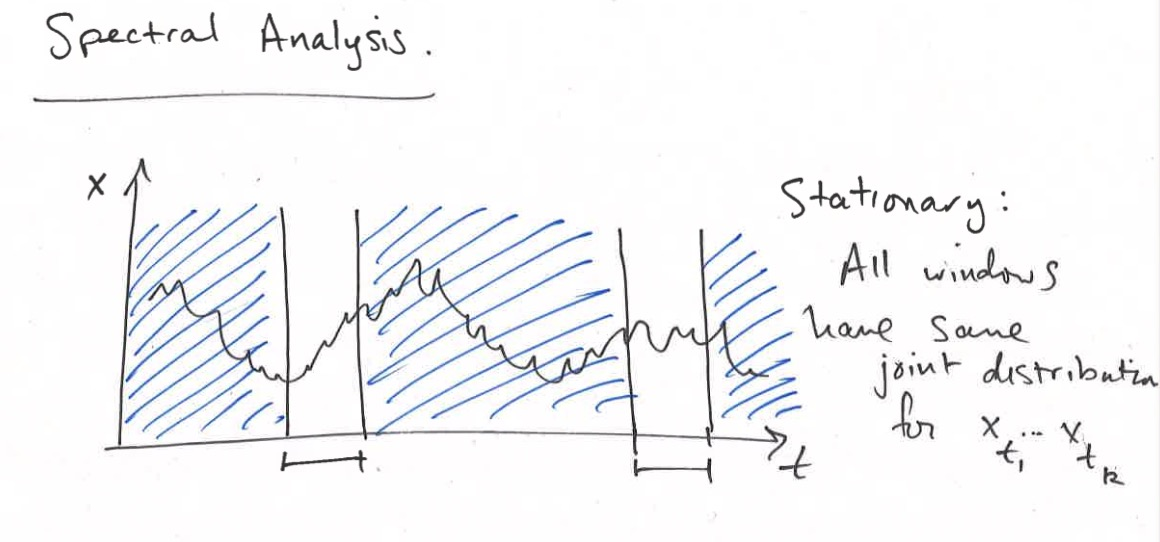
\includegraphics[scale=0.3]{images/Screenshot 2024-04-29 at 08.36.41.jpg}
\centering
\end{figure}


\underline{Question:} Is the following time series stationary:\\
    \[X_t = R \cdot \cos(t+ \phi) + \varepsilon_t\] 
\begin{itemize}
    \item[] Let $R>0$ be a positive random variable.
    \item[] Let $\phi \in [0, 2\pi]$ be a uniform random variable
    \item[] Let $\varepsilon_t$ $t \in Z$ (so $t=...,-2-1,0,1,2,...$)
\end{itemize}
\underline{Answer}: It is stationary: Why? 
\begin{itemize}
    \item[] Compare to $W_t = \cos(t)+ \varepsilon_t$ (i.e., $R=1, \phi = 0$ instead of random) $\Rightarrow$ Not-stationary 
\end{itemize}

\begin{figure}[H]
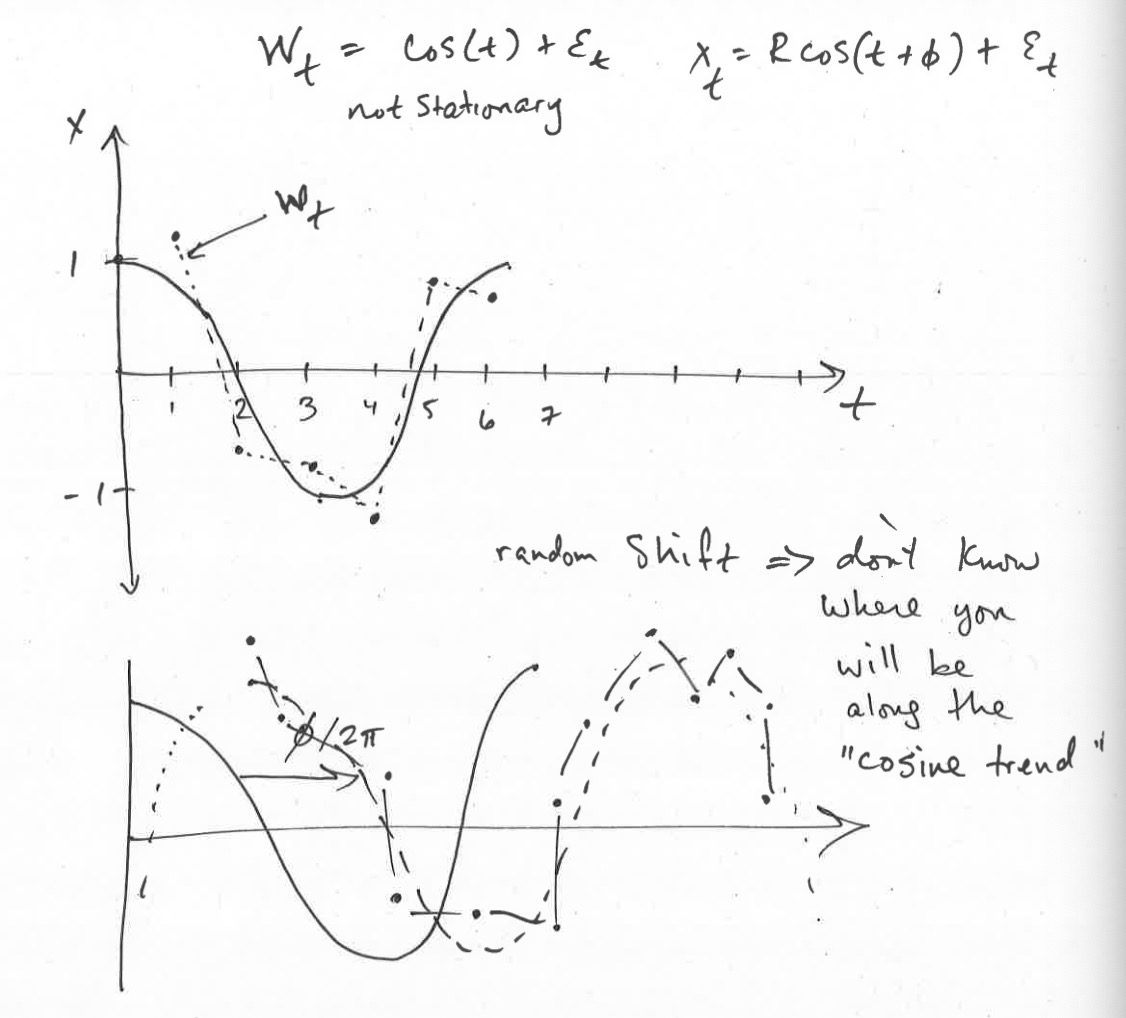
\includegraphics[scale=0.25]{images/Screenshot 2024-04-29 at 08.38.34.jpg}
\centering
\end{figure}

\begin{figure}[H]
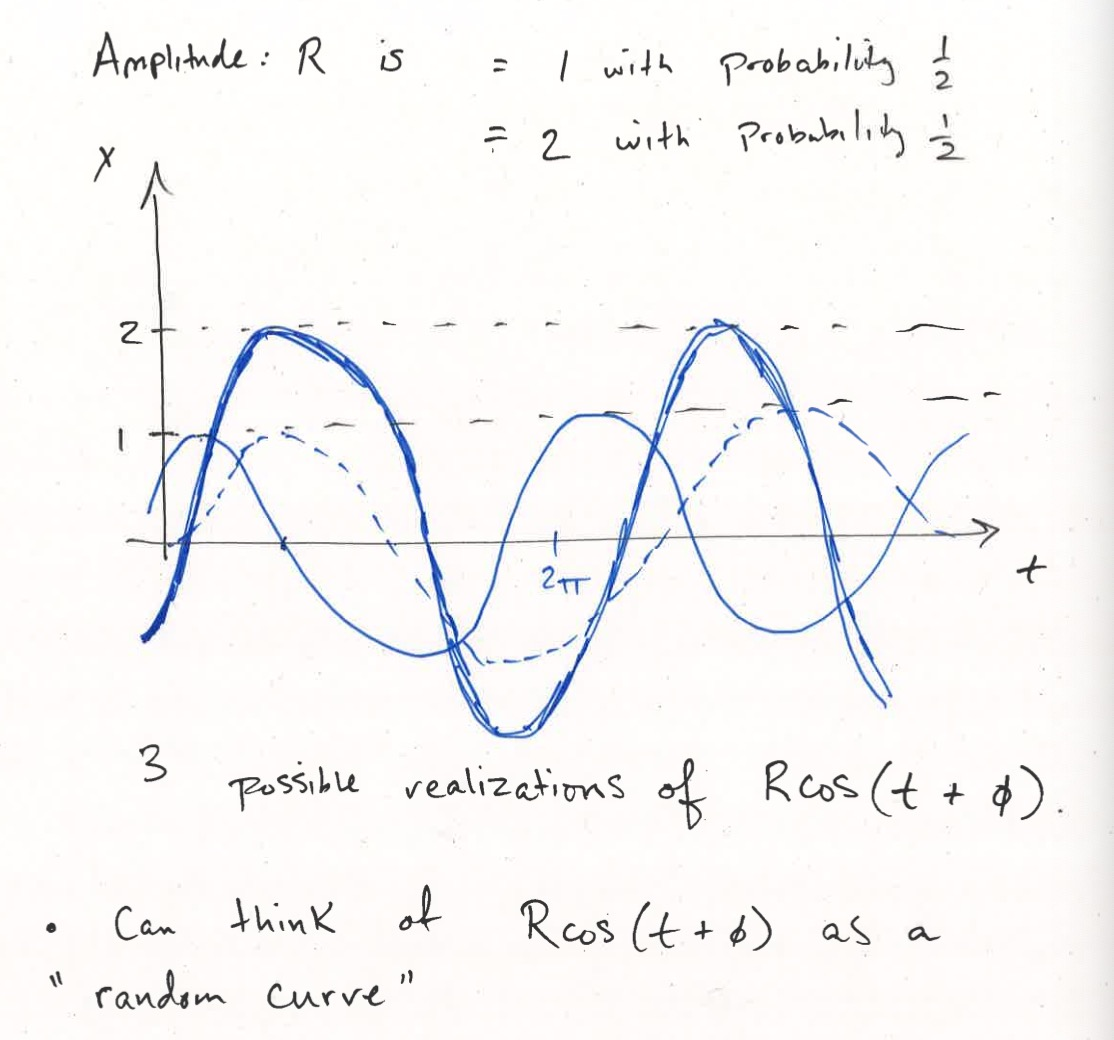
\includegraphics[scale=0.25]{images/Screenshot 2024-04-29 at 08.38.59.jpg}
\centering
\end{figure}

\underline{Question:} Can all stationary time series be decomposed into a sequence of random curves of the form $R(\cos(wt + \phi))$ ? 

\[X_t = \sum_{j=1}^k R_j \cos(w_j t +\phi_j)+Z_t \]
with $w_j$ deterministic frequencies and $R_j, \phi_j$ random amplitudes and phases and $Z_t$ idiosyncratic or iid. 

\underline{Answer:} In a certain sense, yes: \
But have to let $k\rightarrow \infty$ and take a limit in the right way. \\

\noindent
\rule{\linewidth}{0.4pt}
\bigskip

\subsubsection{Spectral Representation Theorem}
For spectral analysis, we again start with a stationary process $\{X_t\}_{t\in \mathbb{Z}}$ and write it in the form 
\begin{align}
    X_t=\mu+\int_0^\infty \left[\alpha(\omega) \cos(\omega t) + \delta(\omega) \sin(\omega t) \right] d\omega, \quad \forall t \in \mathbb{Z} \label{SP1}
\end{align}


A priori, it is not obvious that such decomposition (\ref{SP1}) always exists. The \textbf{spectral representation theorem} however answers this in the affirmative. How can sine and cosine functions (which have a very rigid periodic structure) reconstruct a function (i.e. the time series) that does not (necessarily) have the same regular periodic structure? For intuition, we illustrate this phenomenon using the (scaled) Gaussian kernel function: \[f(x)=\frac{1}{\sqrt{2\pi}}e^{-\frac{x^2}{2}} \]
We want to approximate this function using sine and cosine functions. Recalling that we can write $e^{i\omega j} = \cos(\omega j) + i \sin(\omega j)$, we want to write \[f(x) \approx \frac{1}{N} \sum_{j=0}^{N-1}a_j e^{i2\pi\frac{1}{N} x} \] i.e. as a linear combination of N periodic functions of different frequency. Finding the appropriate weights $a_j$ is called calculating the \textbf{Fourier transform} of $f$. One can show that for $N\rightarrow\infty$, one is able to perfectly reproduce $f$\footnote{More precisely, $\sin(\pi n x)$ and $\cos(\pi nx)$ for $n \in \mathbb{N}$ form a basis for the space of square integrable functions}; for $N$ finite, there will be an approximation error. As $N$ increases, the approximation error decreases: 

\begin{figure}[H]
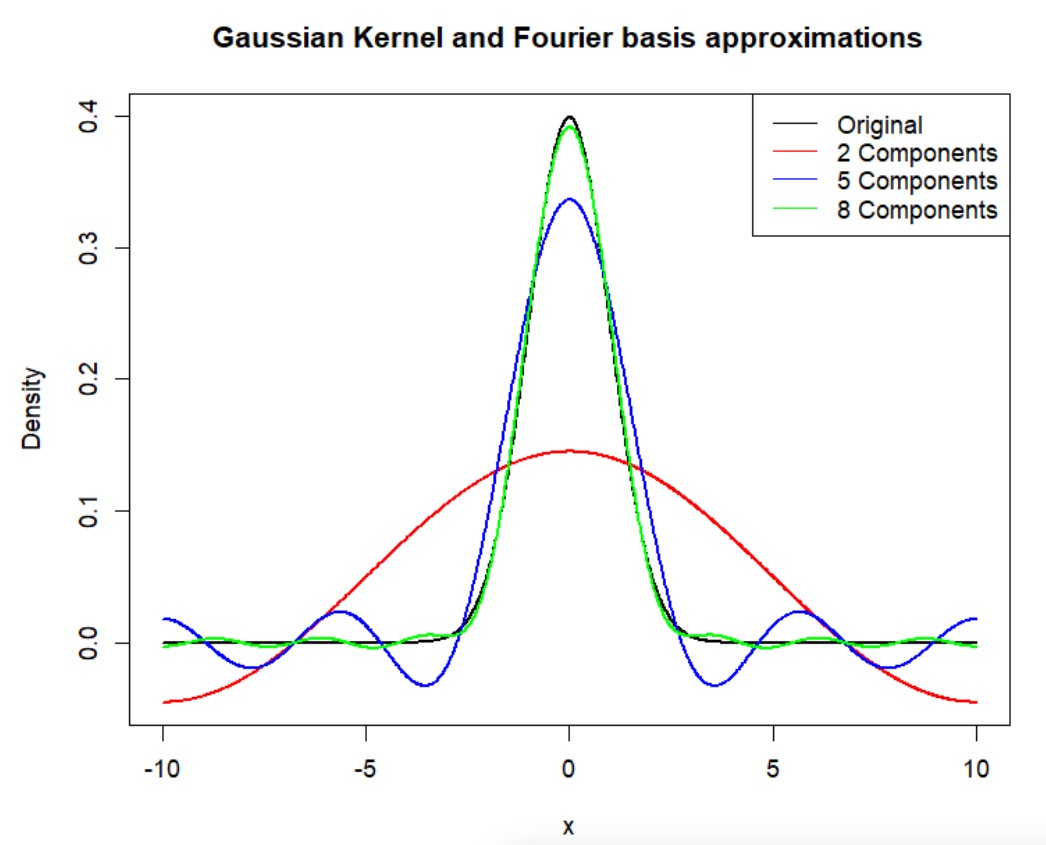
\includegraphics[scale=0.3]{images/Screenshot 2024-05-06 at 09.35.47.jpg}
\centering
\caption{Successive approximation of the gaussian kernel using a Fourier basis. The global approximation error decreases as we increase the number of basis functions}
\end{figure}

How does this relate to time series? Any time series $\{X_t\}_{t\in \mathbb{Z}}$
 can be interpreted as points subsampled from a continuous curve $\{X_t\}_{t\in \mathbb{R}}$. It is possible to define the Fourier transform for both functions on $\mathbb{R}$ (i.e. with uncountable support) and for discrete series (e.g. deterministic time series), simply by exchanging summation and integration. The interpretation of these operations is similar.\\

 Modelling time series differs from function approximation (as above) in that randomness is involved. Hence, rigorously speaking, one cannot apply the above considerations directly to $\{X_t\}_{t\in \mathbb{Z}}$. The appropriate generalization of the Fourier decompositions to random series is the already mentioned spectral representation theorem, stating that any weakly stationary time series can be written as \[X_t=\mu+\int_0^\infty \left[\alpha(\omega) \cos(\omega t) + \delta(\omega) \sin(\omega t) \right] d\omega, \quad \forall t \in \mathbb{Z}\]
 Here, the \textbf{"coefficient functions"} $\alpha(\cdot)$ \textbf{and} $\delta(\cdot)$ \textbf{are random} with the property that, for any frequencies $0<\omega_1<\omega_2<\omega_3<\omega_4<\pi$, the random variables $\int_{\omega_1}^{\omega_2}\alpha(\omega) d \omega $ and $\int_{\omega_3}^{\omega_4}\alpha(\omega) d \omega $, as well as $\int_{\omega_1}^{\omega_2}\delta(\omega) d \omega $ and $\int_{\omega_3}^{\omega_4}\delta(\omega) d \omega $ are uncorrelated. Also, $\alpha$ and $\delta$ are uncorrelated. So, instead of decomposing the process into random independent components at different times, we decompose it into (somewhat) independent components of different frequencies!

\subsection{Key Concepts}
Recall again the definition of the autocovariance function of a stationary process: \[
\gamma(k):=\mathbb{E}[(X_t-\mu)(X_{t-k}-\mu)] \quad \forall k\in \mathbb{N}
\]
We can apply the (discrete) Fourier transform operator to this (discrete) function: \[
f(\omega):=\frac{1}{2\pi} \sum_{j=-\infty}^\infty \gamma(j) e^{-i\omega j}
\] \

because $e^{-i\omega k} = \cos(\omega k) + i \sin(\omega k)$ and $\gamma(k) = \gamma(-k)$ so the "$\sin$" terms cancel out. \\



This new function $f(\cdot)$ is called the \textbf{spectral density} or \textbf{spectrum} of $\{X_t\}_{t\in \mathbb{Z}}$. Since $\gamma(k)=\gamma(-k)$, and using some basic properties of the sine and cosine functions, the spectral density simplifies to: \[
f(\omega)=\frac{1}{2\pi}\{\gamma(0) + 2\sum_{j=1}^\infty \gamma(j) \cos(\omega j)\}
\]

\textbf{Example 1.}\\

The spectrum for:
\begin{enumerate}
    \item White noise: \[
    f(\omega) = \frac{\sigma_Z^2}{2\pi}
    \]
    \item MA(1): \[
    f(\omega)=\frac{1}{2\pi}(1+\theta^2+2\theta\cos(\omega))\sigma_Z^2
    \]
    \item for ARMA(p,q), i.e. $X_t=\mu+\phi_1 X_{t-1}+\cdots+\phi_p X_{t-p} + \epsilon_t + \theta_1 \epsilon_{t-1} + \cdots +\theta_q \epsilon_{t-q} $, one can show that \[
    f(\omega)=\frac{\sigma_Z^2 \prod_(j=1)^q(1+\eta_j^2-2\eta_j \cos(\omega)) }{2\pi \prod_{j=1}^p(1+\lambda_j^2-2\lambda_j\cos(\omega)) }
    \] where $\eta_j$ and $\lambda_j$ are the inverted roots of the characteristic polynomials of the MA and AR parts, respectively.
\end{enumerate}

We have defined the spectral density as a function of the autocorrelations, i.e. the latter implying the former. Actually, both are equivalent, meaning that one can also back out again the autocorrelations from the spectral density: \[
\gamma(k)=\int_{-\pi}^\pi f(\omega) e^{i\omega k} d\omega
\]
This mathematical fact is known in Analysis as the Fourier inverse \footnote{More precisely, for a given function $g$, we can define its Fourier transform $\hat{g}$ as \[
\hat{g}=\frac{1}{2\pi} \int_{-\infty}^\infty g(x)e^{-ix\omega} dx
\] The Fourier inverse theorem states that the converse is also possible: \[
g(x) = \int_{-\pi}^\pi \hat{g}(\omega)e^{ix\omega}d\omega
\]
}. Note that this implies:\[
\gamma(0) = \int_{-\pi}^\pi f(\omega) d\omega
\]
i.e. the variance of the process equals the integral of the spectrum on $[-\pi,\pi]$. Put differently, one can explain the total variance of the process using the information provided by the full spectrum. Actually, \textbf{this result generalizes in a useful way}: the \textbf{part of the variance that is due to frequencies less than} $\omega_1$ equals \[
\int_{-\omega_1}^{\omega_1}f(\omega)d\omega=2\int_0^{\omega_1} f(\omega)d\omega \label{SP2}
\] where the equality comes from the fact that $f(\omega)=f(-\omega)$

\bigskip
\textbf{Example 2.} Let us illustrate what this means in a toy example: consider the process defined as \[
X_t=\sum_{j=1}^M [\alpha_j \cos(\omega_j t) + \delta_j \sin(\omega_j t)]
\] i.e. a discretized version of (\ref{SP1}), using only a finite number of frequencies $0<\omega_1<\cdots<\omega_M<\pi$. The sequences $\{\alpha_j\}_{j=1}^M, \{\delta_j\}_{j=1}^M$ are assumed to be serially uncorrelated and mutually independent with $Var(\alpha_j)=Var(\delta_j)=\sigma_j^2$. Then:\footnote{Recall that $\sin^2(x)+\cos^2(x)=1$} \[
Var(X_t)=\sum_{j=1}^M \sigma_j^2 [\cos^2(\omega_j t)+ \sin^2 (\omega_j t)]=\sum_{j=1}^M \sigma_j^2
\] Hence the part of total variance due to cycles of frequencies less than or equal to $\omega_j$ is $\sum_{j=1}^i \sigma_j^2$ \
How do we use this? Due to (\ref{SP2}), we know that the portion of variance attributable to frequencies in $[\omega_1, \omega_2]$ is given by $2\int_{\omega_1}^{\omega_2}f(\omega)d\omega $. This mean that the area under the graph $f(\cdot)$ between $\omega_1$ and $\omega_2$ is indicative of the importance of the corresponding frequencies for the process overall. If this area is large, then a lot of variance is generated by these frequencies, indicating some seasonality in that area.\\

How do we estimate this? Directly estimating $\gamma(\cdot)$ for all periods and plugging it into $\frac{1}{2\pi}\sum_{j=-\infty}^\infty \gamma(j)e^{-i\omega j} $ is not possible, as we only have finitely many observations. Even the truncated version, i.e. \[ 
\hat{f}(\omega):=\frac{1}{2\pi}\left[ \hat{\gamma}(0)+2\sum_{j=1}^{T-1} \hat{\gamma}(j)\cos(\omega j) \right]
\] is impractical, as we need to estimate just as many parameters as we have observations. One could truncate this series to include fewer terms (a fixed number $M$). Alternatively, one could estimate the parameters of the underlying process in the time domain (i.e. ARMA model estimation), and calculate the implied covariances. Other methods include the smoothed periodogramm and kernel-based methods.

\subsection{Application}

We apply this methodology to US manufacturing data, using the FED's monthly seasonally unadjusted monthly index of production. We calculate the spectrum of the raw series: 

\begin{figure}[H]
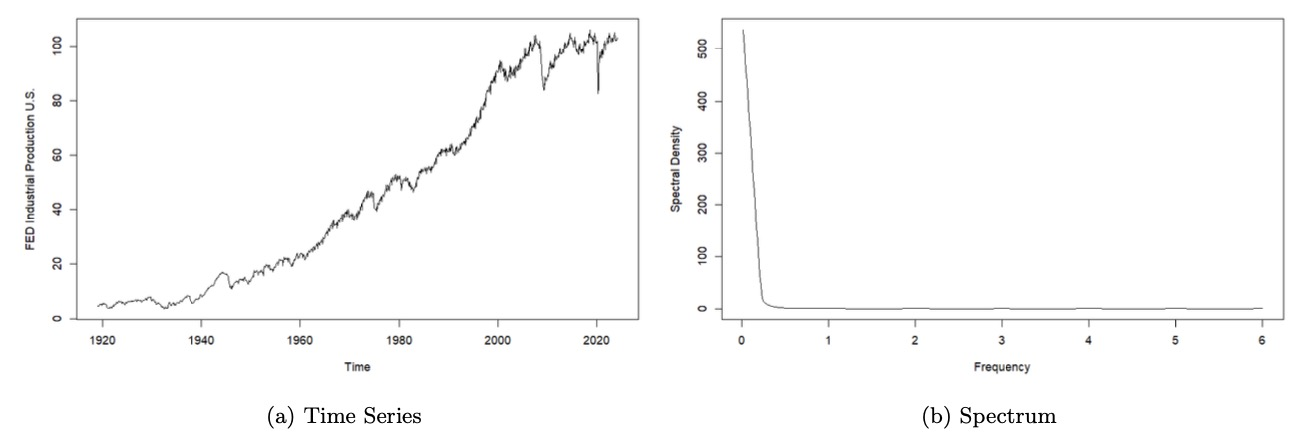
\includegraphics[scale=0.4]{images/Screenshot 2024-05-06 at 10.37.34.jpg}
\centering
\end{figure}

This does not yield meaningful results, as the method requires a stationary time series. In this case, the low-frequency (i.e. long-term) cycles induced by the uptrend dominate everything else. We therefore re-apply this method to the ime series of log-differences: 

\begin{figure}[H]
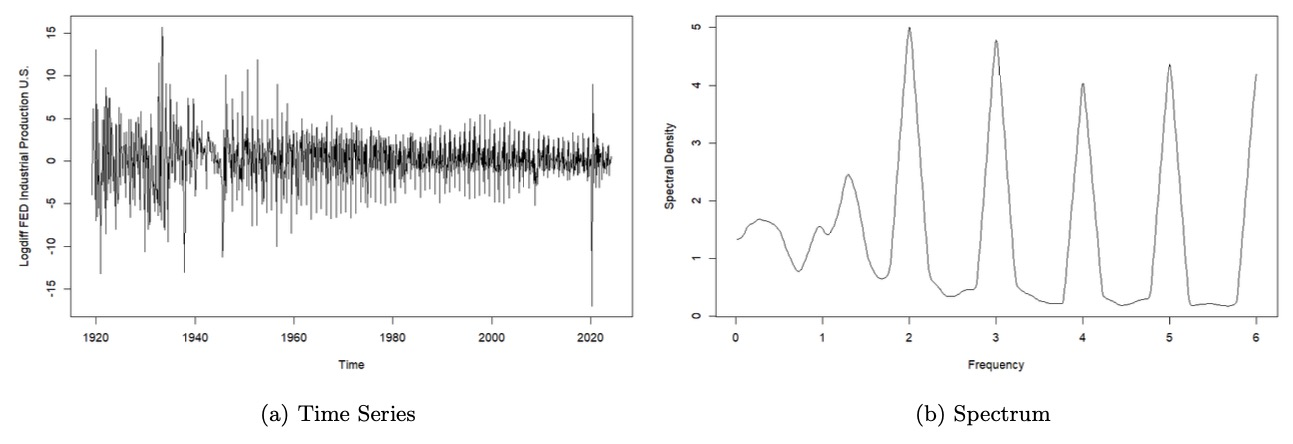
\includegraphics[scale=0.4]{images/Screenshot 2024-05-06 at 10.39.09.jpg}
\centering
\end{figure}

This gives an interpretable spectral density. Recall that the area under the curve represents the portion of total variance due to these frequencies. A spike at a certain frequency therefore means that it is important to the time series. In our case, we observe several spikes in the low frequencies (first and second bump), corresponding roughly to the business cycle (2.5 - 3 years) and a 12-month cycle. The remaining higher frequencies could potentially come from intra-year seasonalities, e.g. calendar effects. If we consider a year-on-year difference (log), then virtually all the seasonal components vanish, with only the business cycle frequency remaining: 
\begin{figure}[H]
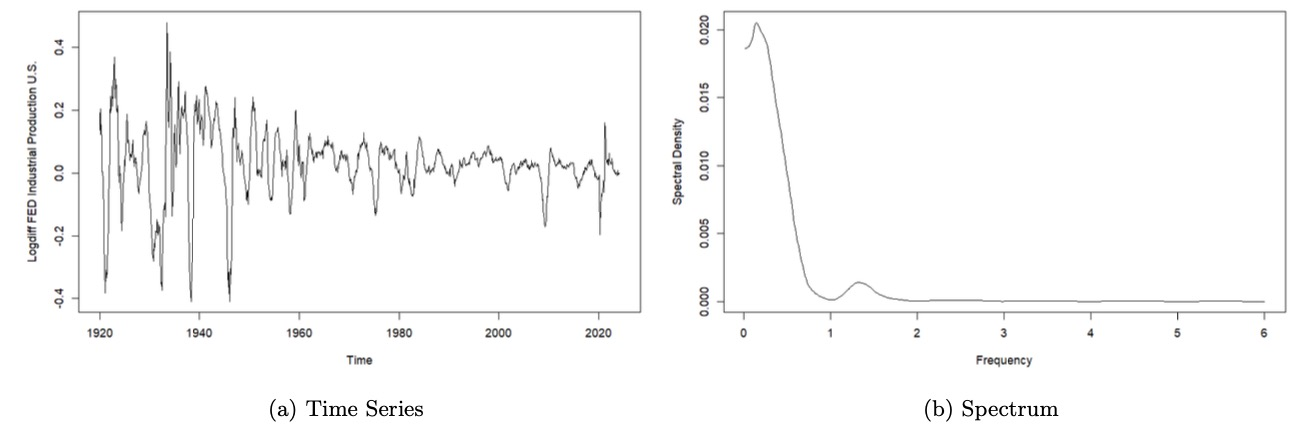
\includegraphics[scale=0.4]{images/Screenshot 2024-05-06 at 10.41.41.jpg}
\centering
\end{figure}




\subsection{Spectrum Calculation for White Noise Process}
\begin{align*}
    f(\omega)&=\frac{1}{\pi} \sum_{k=-\infty}^\infty \gamma(k) e^{-i\omega k}\\
    \gamma(0) & \neq 0 \quad \text{but $\gamma_k = 0$ \quad $\forall k\neq0$} \\
    &+ \frac{1}{\pi} \sum_{k\neq 0} \underbrace{\gamma(k)}_{=0} e^{-i\omega k} \\
    &= \frac{1}{\pi} \gamma(0)\\
    &= \frac{1}{\pi}var(X_t)
\end{align*}

\begin{figure}[H]
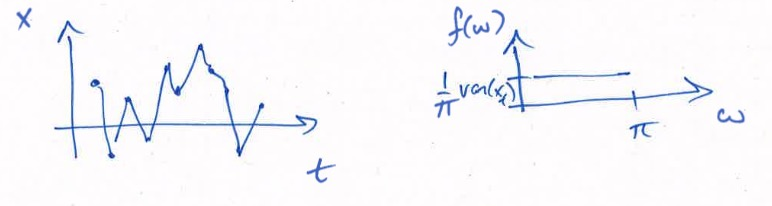
\includegraphics[scale=0.4]{images/Screenshot 2024-04-29 at 08.42.56.jpg}
\centering
\end{figure}



\subsection{Spectrum Calculation for MA process}
\[X_t=\varepsilon_t + \theta \varepsilon_{t-1}\]
what is $\gamma(k)$?
\begin{align*}
    \gamma(1)&=cov(\varepsilon_t+\theta \varepsilon_{t-1}, \varepsilon_{t-1} \theta \varepsilon_{t-2} \\
    &= cov(X_t, _{t-1})\\
    &= cov(\varepsilon_{t}, \varepsilon_{t-1})+cov(\theta \varepsilon_{t-1}, \varepsilon_{t-1}) + cov(\varepsilon_{t}, \theta \varepsilon_{t-2}+cov(\theta \varepsilon_{t-1}, \theta \varepsilon_{t-2}\\
    &= \theta cov(\varepsilon_{t-1},\varepsilon_{t-1}) &&\text{(all other terms $=0$)}\\
    &= \theta var(\varepsilon_{t}\\
    \gamma(0)&= cov(\varepsilon_{t}, \theta \varepsilon_{t-1}, \varepsilon_{t} + \theta \varepsilon_{t-1}) \\
    &= (1+\theta^2)var(\varepsilon_{t}) \\
    \gamma(2)&=0 &&{\gamma(k)=0 \text{\quad} \forall |k|\geq 2 } \\
    \Rightarrow f(\omega) &= \frac{1}{\pi} [ 1 + \theta^2 + 2 \theta \cos(\omega) ]var(\varepsilon_t)
\end{align*}

How to estimate $f(\omega)$ given data $X_1,...,X_T$?
\begin{align*}
    f(\omega) =\frac{1}{\pi} [ \gamma(o) + 2\sum_{k=1}^\infty \gamma(k) \cos \omega k] 
\end{align*}

Two options for $\hat{f}$: 
\begin{enumerate}
    \item Truncate $\sum_{k=1}^\infty$ to $\sum_{k=1}^\mu$ for $M<<T$ to avoid degeneracy ($M=T$ doesn't work)
    \item Smoothed periodogram
\end{enumerate}

\underline{Periodogram}:
\begin{align*}
    I(\omega) &= \frac{1}{\pi T} \left | \sum_{t=1}^T X_t e^{i\omega t}\right |^2\\
    &= \frac{1}{\pi T} \left[ \left| \sum_{t=1}^T \cos(\omega t)X_t + i \sin(\omega t)X_t \right |^2 \right]
\end{align*}

\underline{Smoothed periodogram}:  \\

Smoothed version of $I(\omega)$\\

The value of the periodogram is 
\begin{align*}
    \underset{T\rightarrow\infty}{lim} E\left[I(\omega) \right] = f(\omega)
\end{align*}

Unfortunately, 

\[\underset{T \rightarrow \infty}{lim} var(I(\omega)) \neq 0 \]

But with Smoothing + the property that 
\[I(\omega_1) \overset{\ind}{\approx} I(\omega_2) \text{
\quad "$\overset{\ind}{\approx}$" means approximately independent. 
} \]


\[\Rightarrow \frac{1}{2a} \int_{\omega_0 - a}^{\omega_0 + a} I(\omega)d\omega \approx f(\omega_0) \text{\quad for a small $T$ with high probability.}\]



\underline{Spectral methods continued}:
\bigskip
Let $X_t, t=1,...,T$ be observations from a stationary time series. \\

Two objects:
\begin{enumerate}
    \item Spectral density: $f(\omega)=\frac{1}{\pi} \sum_{k=-\infty}^\infty \gamma(k) e^{\omega k \sqrt{-1}}$, where $\gamma(k) = cov(X_t, X_{t-k})$
    \item Periodogram: $I(\omega) = \frac{1}{\pi T} \left| \sum_{t=1}^T X_t e^{t\omega \sqrt{-1}} \right|^2$
\end{enumerate}

\underline{Properties}: 
\begin{itemize}
    \item $\underset{T\rightarrow\infty}{lim} E\left[I(\omega) \right] = f(\omega)$ 
    \item $\underset{T\rightarrow\infty}{lim} Var(I(\omega))\neq0$
    \item "For $\omega_1 \neq \omega_2$, $I(\omega_1)$ and $I(\omega_2)$ become approximately independent for large T
    \begin{itemize}
        \item[] $\Rightarrow$ Law of large numbers effect
        \item[] Smoothed periodogram can estimate $f(\omega)$ 
    \end{itemize}
\end{itemize}

\subsection{Variance Estimation and Inference via Periodogram}

\textbf{\underline{Inference problems:}}

\begin{itemize}
    \item Estimating a mean 
    \[X_t=\mu + \varepsilon_t\]
    \[\hat{\mu}= \frac{1}{T} \sum_{t=1}^T X_t\]
    \item \textbf{Question}: How to compute a confidence interval for $\mu$? 
    \item A generalization of this problem is: estimate a regression with two time series \[y_t=\alpha+\beta X_t +\varepsilon_t\]
    \item[] $\rightarrow \hat{\beta}$ via OLS leads to question: How to compute a confidence interval? 
    \item \textbf{Answer}: variance of $\hat{\mu}$ is encoded in spectral density at 0
    \item Why? $X_t = \mu + \varepsilon_t$ $\varepsilon_t$ mean $0$ but possibly dependent.
    \begin{itemize}
        \item[] $\hat{\mu}= \frac{1}{T} \sum_{t=1}^T X_t$
        \begin{align*}
            var(\hat{\mu}) &= var(\frac{1}{T} \sum_{t=1}^T X_t) \\
            &= var(\frac{1}{T} \sum_{t=1}^T \varepsilon_t) \\
            &= \frac{1}{T^2} \sum_{s,t=1}^T cov(\varepsilon_s, \varepsilon_t) \\
            &\text{Let $\gamma$ be autocovariance function of $\varepsilon_t$} \\
            &\approx \frac{1}{T^2} \left[ \sum_{s=1}^T cov(\varepsilon_s, \varepsilon_s) + \sum_{s=2}^T cov(\varepsilon_{s}, \varepsilon_{s-1}) +  \sum_{s=2}^T cov(\varepsilon_{s-1}, \varepsilon_{s})  + \sum_{s=3}^T cov(\varepsilon_{s}, \varepsilon_{s-2}) + ...\right] \\
            &=\frac{1}{T^2} \left[\sum_{s=1}^T \gamma(0) +  \sum_{s=2}^T \gamma(1) + \sum_{s=2}^T \gamma(-1) + \sum_{s=3}^T \gamma(2) + ... \right] \\
            var(\hat{\mu}) &= \frac{1}{T^2} \left[T\gamma(0) + (T-1)\gamma(1) + (T-1)\gamma(-1) + (T-2)\gamma(2) + ... \right]\\
            &\approx \frac{1}{T^2} \left[T(\gamma(0)+ \gamma(1)+\gamma(-1)+\gamma(2)+...) \right]\\
            &= \frac{1}{T} \left[\gamma(0)*1 + \gamma(1)*1+\gamma(-1)*1+\gamma(2)*1 +...\right] \\
            &= \frac{1}{T} \left[\gamma(0)e^{-0*0*\sqrt{-1}} + \gamma(1) e^{-0*1*\sqrt{-1}} + \gamma(-1) e^{-0*-1*\sqrt{-1}} + \gamma(2) e^{-0*2*\sqrt{-1}}+... \right] \\
            &=\frac{1}{T} \sum_{k=-\infty}^\infty \gamma(k) e^{-0*k*\sqrt{-1}} \\
            &= \frac{\pi}{T} f(0) \text{\quad (-or- $f(\omega)$ at $\omega=0$)} \\
        \end{align*}
        \item[] \fbox{$\frac{\pi}{T}f(0)$} clearly written
        \item Estimated with smooth periodogram
        \begin{itemize}
            \item[] $smooth(\frac{\pi}{T} I(0))$ estimates $var(\hat{\mu})$
        \end{itemize}
    \end{itemize}
\end{itemize}

\textbf{\underline{Procedure for estimating mean}}
\begin{itemize}
    \item Have: $X_t = \mu + \varepsilon_t$
    \item Calculate $\hat{\mu} = \frac{1}{T} \sum_{t=1}^T X_t$
    \item Know $var(\hat{\mu}) \approx \frac{\pi}{T} f(0)$ where $f(\omega)$ is spectral density of $\varepsilon_t$
    \item 
\end{itemize}
To estimate $var(\hat{\mu})$ from periodogram with $\hat{\varepsilon}_t=X_t-\hat{\mu}$ \[I(\omega)=\frac{1}{\pi T} \left| \sum_{t=1}^T \hat{\varepsilon}_t e^{t\omega \sqrt{-1}} \right|^2 \]
Choose Smoothing window: h $\rightarrow$ important, difficult in practice, usually choose $h=\frac{1}{\sqrt{T}}$\\

\quad h must be between $0$ and $\pi$
\begin{align*}
    \hat{f}(0) &= \frac{1}{h} \int_0^h I(\omega)d\omega \\
    \hat{var}(\hat{\mu}) &= \frac{\pi}{T}\hat{f}(0)
\end{align*}




\section{Non-linear Time Series}
Technically, no official definition of nonlinear time series, but sometimes, there is an obvious choice for what to call linear or nonlinear. \\

For time series like \[X_t = f(X_{t-1} ... X_{t-p}) + \varepsilon_t \]
\begin{itemize}
    \item if $f(X_{t-1} ... X_{t-p})$ is something like $ =\alpha_1 X-{t-1} + ...+ \alpha_p X_{t-p}$ call this linear. Otherwise, nonlinear.
\end{itemize}
ARMA models are considered linear by everyone. 

\subsection{Threshold AR models}
Idea: Glue together two different AR models.\\

Simplest way is depending on value of $X_{t-1}$:
\begin{subequations}
\begin{empheq}[left = {X_t=\empheqlbrace}]{align*} 
    &v_1 + a_1X_{t-1} + \sigma_1 \varepsilon_t &&\text{if $X_{t-1} < r$} \\
    &v_2 + a_2 X_{t-1} 1 \sigma_2 \varepsilon_t &&\text{if $X_{t-1}\geq r$}
\end{empheq}
\end{subequations}

\textcolor{red}{ Graph}

Estimation: Choose a distribution for $\varepsilon_t$ (like $N(0,1)$) and do maximum likelihood. \[\rightarrow \hat{v}_1,\hat{v}_2,\]

\section{Impulse Response Functions and Multivariate Time Series}
\subsection{Impulse Response Function}
What is an impulse response function? \\
\begin{figure}[H]
    \centering
    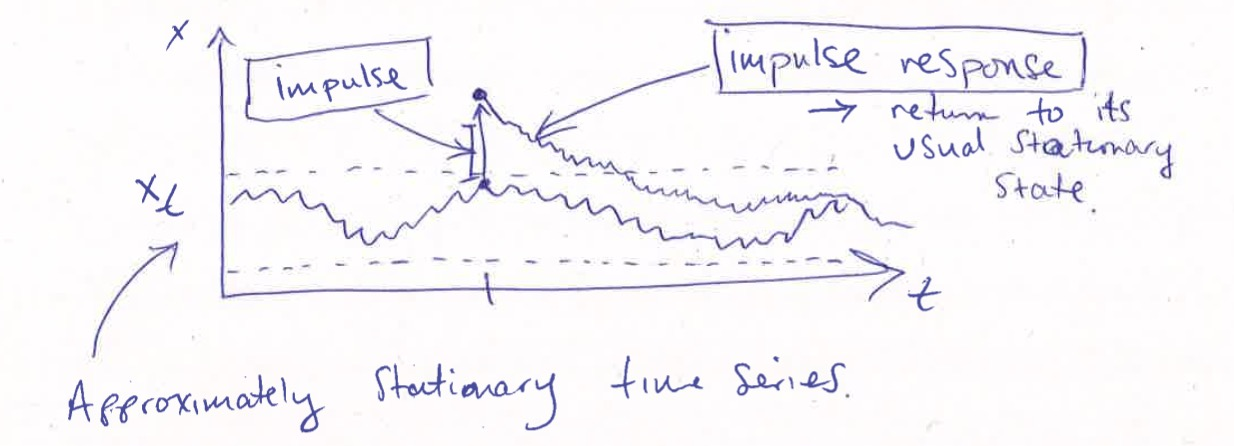
\includegraphics[width=0.8\linewidth]{images/Screenshot 2024-05-21 at 18.13.20.jpg}
    \caption{Impulse Response Function}
\end{figure}


\noindent
\rule{\linewidth}{0.4pt}
Will work towards a definition where 
\begin{align*}
    &\fbox{IRF(r)} \quad \text{is related to (or equal to)} \\
    % & \frac{ \partial X_{t+r} }{ \partial \varepsilon_t }\\
\end{align*}

Suppose $X_t=\alpha + \varepsilon_t +\theta_1 \varepsilon_{t-1} + \theta_2 \varepsilon_{t-2}$ 
\begin{itemize}
    \item This is a MA(2) process with parameters $\alpha, \theta_1, \theta_2$
    \item Stationary
    \item Can define $x_t$ if you know all $\varepsilon_t$s 
    \begin{align*}
    IRF(r)&=\frac{\partial x_{t+r}}{\partial \varepsilon_t}\\
    IRF(0)&= \frac{d(\alpha+\varepsilon_t+\theta_1 \varepsilon_{t-1}+\theta_2 \varepsilon_{t-2}}{\partial \varepsilon_t}\\ 
    &=1\\
    IRF(1)&=\theta_1\\
    IRF(2)&=\theta_2
    \end{align*}
\end{itemize}

IRFs for more general models.
\begin{itemize}
    \item Stationary time series are almost always approximated by moving averages (MA) series.
    \item Mathematically, there is a MA($\infty$) representation of a stationary time series in many cases. 
    \item Example: AR(1) model:
    \[
    X_t = \alpha + \rho X_{t-1}+\varepsilon_t
    \]
    \begin{itemize}
        \item Invert backshift operator: $X_{t-1}=BX_t$ \[
        X_t= \alpha+\rho BX_t +\varepsilon_t
        \]\[
        \Rightarrow (1-pB)X_t=\alpha+\varepsilon_t
        \]
    \end{itemize}
    \item If $|p|<1$ its possible to invert $(1-pB)$ (why? if the roots of the "polynomial in B" are outside unit circle, then you can "divide")
    \begin{itemize}
        \item Solve $1-\rho B = 0 \longrightarrow B = \frac{1}{\rho} > 1$ if $0<\rho<1$
    \end{itemize}
\end{itemize}
\begin{align*}
    X_t= \alpha+\rho BX_t +\varepsilon_t\\  
    \Rightarrow (1-pB)X_t=\alpha+\varepsilon_t \\
    \text{if } |p|<1 \quad \text{then}\\
    (1-\rho B)^{-1} = ?
\end{align*}
Simpler example 
\begin{align*}
    \frac{1}{1-\frac{1}{4}} &= 1+\frac{1}{4} + \frac{1}{16} + \frac{1}{64} + \cdots \\
    &= \frac{4}{3}
\end{align*}
\underline{Define}: \[
(1-\rho B)^{-1}= 1+\rho B + \rho^2 B^2 + \rho^3 B^3 + \cdots
\]
Theorem: if $X_t$ is sufficiently well behaved (stationary etc.) and $|p|<1$ then \[
(1-\rho B)^{-1}X_t= (1+\rho B + \rho^2 B^2 + \rho^3 B^3)X_t
\]
and $(1-\rho B)^{-1} (1-\rho B) X_t = X_t$ (cancellation property).

\begin{align*}
    X_t &= \alpha+ \rho B X_t + \varepsilon_t\\
    (1-\rho B) X_t &= \alpha + \varepsilon_t \\
    (1-\rho B)^{-1}(1-\rho B) X_t &= (1-\rho B)^{-1} (\alpha + \varepsilon_t)\\
    \Rightarrow X_t &= \alpha + \varepsilon_t + \rho B(\alpha + \varepsilon_t)+ \rho^2 B^2(\alpha+\varepsilon_t) + \cdots
\end{align*}
The point: Now you can calculate impulse responses
\begin{align*}
    \frac{\partial X_t}{\partial \varepsilon_{t-r}} &= \frac{\partial}{\partial\varepsilon_{t-r}} \rho^r (\alpha+\varepsilon_{t-1}) \\
    &= \frac{\partial}{\partial \varepsilon_{t-r}} \rho^r \varepsilon_{t-r} \\
    &= \rho^r\\
    IRF(r) &= \rho^r
\end{align*}
$\rho^r$ measures "where $X_t$ would have been"
\begin{figure}[H]
    \centering
    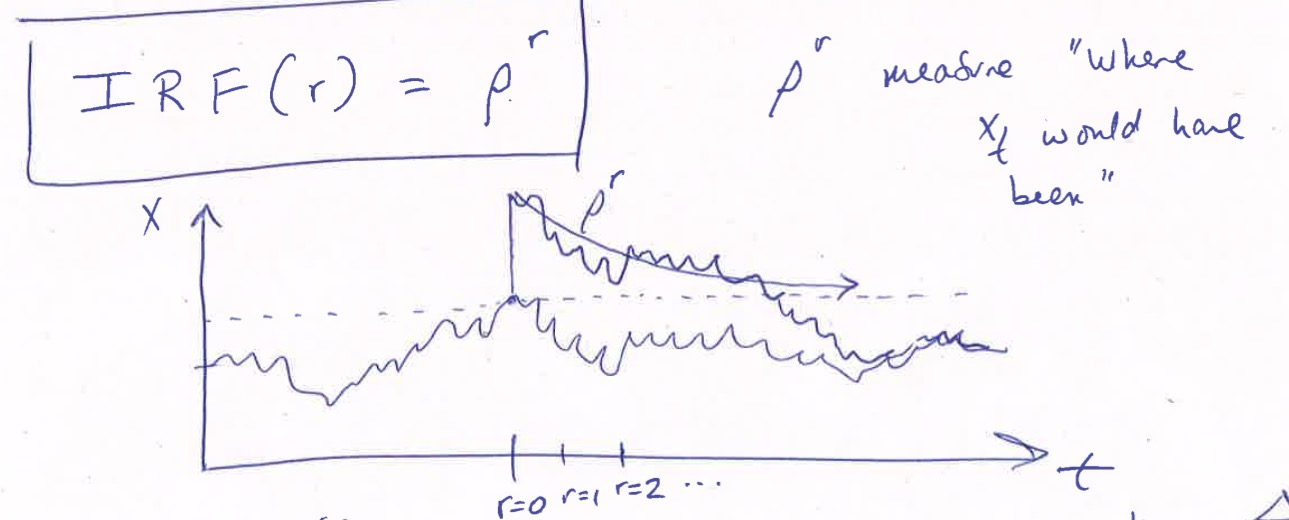
\includegraphics[width=0.75\linewidth]{images/Screenshot 2024-05-21 at 18.16.58.jpg}
\end{figure}

In ARMA(1,1)
\begin{align*}
    X_t &= \alpha + \rho X_{t-1} + \varepsilon_t + \theta \varepsilon_{t-1} \\
    (1-\rho B)X_t &= \alpha + \varepsilon_t + \theta \varepsilon_{t-1} \\
    X_t &= (1-\rho B)^{-1} (\alpha + \varepsilon_t + \theta \varepsilon_{t-1}) \\
&= 1\cdot (\alpha + \varepsilon_t + \theta \varepsilon_{t-1} + \rho B (\alpha + \varepsilon_t + \theta \varepsilon_{t-1}) + \rho^2 B^2(\alpha + \varepsilon_t + \theta\varepsilon_{t-1})\\
&\text{get IRF that way}
\end{align*}

\subsection{Multivariate Time Series}

\rule{\textwidth}{0.4pt}
\bigskip
\textbf{\underline{Book: Chapter 13}}\\

Observations are often taken simultaneously on two or more time series. For such multivariate data, it may be helpful to develop a multivariate model to describe the interrelationships among the series. However, the model-building process is much more difficult than for univariate models. Multivariate models are more vulnerable to misspecification, this emphasizes the importance of getting sufficient background information so as to understand the context and identify all relevant variables before starting the modelling process. An iterative approach to model building is generally required. With multivariate time series data, the modelling process is complicated by the need to model the serial dependence \textit{within} each series, as well as the interdependence \textit{between} series. Multivariate forecasts are not always as good as might be expected.\\

One basic question is whether the model should involve a single equation or multiple equations. In multiple regression, for example, the model explains the variation in a \textbf{single response} variable in terms of one or more \textbf{predictor} or \textbf{explanatory} variables. In a single-equation model there should not be any suspicion that the response variable could itself affect the predictor variables, i.e., we assume there is an \textbf{open-loop} system. \

When the 'outputs' affect the 'inputs' there is \textbf{feedback} in a \textbf{closed-loop} system, e.g., wages and prices in a simultaneous equation model. \\

\bigskip
\noindent
\textbf{\underline{Cross-correlation function}}\\

A key tool in modelling multivariate time series is the cross-correlation function. First, look at the bivariate case and the \textbf{cross-variance function} of two time series at the same unit interval and over the same period $(x_1,y_1), \cdots, (x_N, y_N)$, which is defined as \begin{align}
Cov(X_t,Y_{t+k})=\mathbb{E}[(X_t-\mu_x)(Y_{t+k}-\mu_Y)] = \gamma_{XY}(k) \label{cross-cov}
\end{align}
Unlike, the acv.f. this it not an even function. Thus $\gamma_{XY}(k)\neq \gamma_{XY}(-k)$, instead $\gamma_{XY}(k)=\gamma_{YX}(-k)$.\
Useful to standardize the cross-covariance function to produce a function called the \textbf{cross-correlation function}, which is defined as: \[
\rho_{XY}(k)=\frac{\gamma_{XY}(k)}{\sqrt{\gamma_X(0) \gamma_Y(0)}} = \frac{\gamma_{XY}(k)}{\sigma_x \sigma_Y} \label{cross-corr}
\]
\quad where $\sigma_X = \sqrt{\gamma_X(0)}$ denotes the standard deviation of the X-process, and similarly for $\sigma_Y$. This function measures the correlation between $X_t$ and $Y_{t+k}$ and has two properties: 
\begin{enumerate}
    \item $\rho_{XY}(k)= \rho_{YX}(-k)$
    \item $|\rho_{XY}(k)| \leq 1$
\end{enumerate}
Whereas $\rho_X(0), \rho_Y(0)$ are both equal to one, the value of $\rho_{XY}(0)$ is usually \textit{not} equal to one. \\

\begin{equation}
\begin{split}
c_{XY}(k) = & \left\{
\begin{aligned}
    &\sum_{t=1}^{N-k}(x_t-\Bar{x})(y_{t+k}-\Bar{y})/N  &&k=0,1,\cdots, N-1 \\
    & \sum_{t=1-k}^N (x_t-\Bar{x})(y_{t+k}-\Bar{y})/N && k=-1,-2,\cdots,-(N-1)
\end{aligned}
\right.
\end{split}
\end{equation}

and the \textbf{sample cross-correlation function is} \[
r_{XY}(k)= \frac{c_{XY}(k)}{s_X s_Y}
\] \quad where $s_X,s_Y$ are the sample standard deviations.\\
It can be shown that these estimators are asymptotically unbiased and consistent. However, estimators at neighbouring lags are themselves autocorrelated. Furthermore the variances of sample cross-correlations depend on the autocorrelation functions of the two components. In general, the variances will be inflated. Thus it is possible for two series, which are actually uncorrelated, to apparently have large autocorrelation coefficients, which are spurious, in that they arise solely from autocorrelations within the two time series. Solution $\Rightarrow$ one series should first be filtered to convert it to (approximate) white noise and then the same filter is applied to the second series before computing the cross-correlation function.\\

Back to the \textbf{multivariate} case, we redefine the cross-correlation function for an $m$-variate multivariate process, say $\{X_t\}$, where $X_t^T=(X_{1t},X_{2t},\cdots,X_{mt})$. Let $\mu_t$ be the vector of \textbf{mean} values of $X_t$ at time $t$, so that its $i$th component is $\mu_{it}=\mathbb{E}(X_{it})$. Let $\Gamma(t,t+k)$ denote the \textbf{cross-covariance matrix} of $X_t$ and $X_{t+k}$, so that its $(i,j)$th element is the cross-covariance coefficient of $X_{it}$ and $X_{j,t+k}$. A multivariate process is said to be \textbf{second-order stationary} if the mean and the cross-covariance matrices at different lags do not depend on time. Then $\mu_t$ will be a constant, while $\Gamma(t,t+k)$ will be a function of the lag $k$ only, say $\Gamma(k)$. Then the $(i,j)$th element of $\Gamma(k)$, say $\gamma_{ij}(k)$, is given by 
\begin{align}
    \gamma_{ij}(k)=Cov(X_{it},X_{j,t+k})= \mathbb{E}[(X_{it}-\mu_i)(X_{j,t+k}-\mu_j)]
\end{align}
see equation (\ref{cross-cov}). In the stationary case, the set of cross-covariance matrices, $\Gamma(k)$ for $k=0,\pm 1,\pm 2,\cdots$ is called the \textbf{covariance matrix function}. \\
It has rather different properties to the (auto)covariance function in univariate time series in that it is not an even function of lag (as explained above), thus we get \[
\Gamma(k)=\Gamma^T(-k) \quad k=0,\pm1,\pm2,\cdots
\]
Given the covariance matrix function, it is easy to standardize any particular element to find the corresponding cross-correlation and hence construct the set of $(m\times m)$ cross-correlation matrices, $R(k)$ for $k=0,\pm1,\pm2,\cdots$, called zje \textbf{correlation matrix function} of the process. Thus the $(i,j)$th element of $R(k)$ is given by 
\begin{align}
    \rho_{ij}(k)=Corr(X_{it},X_{j,t+k})= \frac{\gamma_{ij}(k)}{\sigma_i \sigma_j}
\end{align}
\quad where $\sigma_i$, the standard deviation of $X_{it}$, can also be expressed as $\sqrt{\gamma_{ii}(0)}$.\\

\noindent
\textbf{\underline{Estimation:}} The sample cross-covariance coefficient of $X_i$ and $X_j$ at lag $k$ is given by

\begin{equation}
\begin{split}
c_{ij}(k) = & \left\{
\begin{aligned}
    &\sum_{t=1}^{N-k} (x_{it} - \bar{x}_i)(x_{j,t+k} - \bar{x}_j)/N & \quad & k = 0, 1, \ldots, N-1 \\
    &\sum_{t=1-k}^{N} (x_{it} - \bar{x}_i)(y_{j,t+k} - \bar{x}_j)/N & \quad & k = -1, -2, \ldots, -(N-1)
\end{aligned}
\right.
\end{split}
\end{equation}

and the \textbf{sample cross-correlation coefficient} is given by
\begin{align}
    r_{ij}(k)=\frac{c_{ij}(k)}{s_is_j}
\end{align}
\quad where $s_i=\sqrt{c_{ii}(0)}$ denotes the sample standard deviation of observations on the $i$th variable

\subsubsection{Vector Autoregressive Models}

Vector Autoregressive Models (VAR) are arguably the most important class of models for \textbf{multiple time-series modelling}.\\

\bigskip
\noindent
\textbf{\underline{VAR(1) models}}\\

With $m$ variables, a natural way to represent them is by means of a $(m\times 1)$ vector $\mathbf{X}_t$ where $\mathbf{X}_t^T=(X_{1t},\cdots, X_{mt})$. For simplicity, first look at $m=2$. For stationary series, we may, without loss of generality, assume the variables haven been scaled to have zero mean. 

\begin{equation}
\begin{array}{r@{}l}
& \left.
\begin{aligned}
    X_{1t} &= \phi_{11} X_{1,t-1} + \phi_{12} X_{2,t-1} + \varepsilon_{1t} \\
    X_{2t} &= \phi_{21} X_{1,t-1} + \phi_{22} X_{2,t-1} + \varepsilon_{2t} \label{eq9}
\end{aligned}
\right\}
\end{array}
\end{equation}


where $\phi_{ij}$ are constants. The two 'error' terms $\varepsilon_{1t}$ and $\varepsilon_{2t}$ are usually assumed to be with noise but are often allowed to be correlated contemporaneously. 
\begin{itemize}
    \item If $\phi_{12}=\phi_{21}=0$ then $X_{1t}$ and $X_{2t}$ are not dynamically correlated $\Rightarrow$ univariate case, analyze separately
    \item If one of $\phi_{12}$ and $\phi_{21}$ is not zero, say $\phi_{12}=0$, but $\phi_{21}\neq 0$, then Equation (\ref{eq9}) reduces to
    \begin{equation}
\begin{split}
& \left.
\begin{aligned}
    X_{1t} &= \phi_{11} X_{1,t-1} + \varepsilon_{1t} \\
    X_{2t} &= \phi_{21} X_{1,t-1} + \phi_{22} X_{2,t-1} + \varepsilon_{2t}
\end{aligned}
\right\}
\end{split}
\end{equation}
        \begin{itemize}
            \item In such a case $X_{1t}$ does not depend on the lagged value of $X_{2t}$. Thus, any causality only goes in one direction.
            \item We can think of $X_{1t}$ as the input and $X_{2t}$ as the output. 
        \end{itemize}
\end{itemize}

\noindent
Equation (\ref{eq9}) can be rewritten in vector form as 
\begin{align}
    \mathbf{X}_t=\Phi \mathbf{X}_{t-1}+ \varepsilon_t \label{vectorForm}
\end{align}
where $\varepsilon_t^T=(\varepsilon_{1t},\varepsilon_{2t})$ and \[\Phi=\begin{pmatrix}
    \phi_{11} & \phi_{12}\\
    \phi_{21} & \phi_{22}
\end{pmatrix}\]

\noindent
Equation (\ref{vectorForm}) looks like an AR(1) model except that $\mathbf{X}_t$ (and $\varepsilon_t$) are now vectors instead of scalars. Since $\mathbf{X}_t$ depends on $\mathbf{X}_{t-1}$ we call this model a \textbf{vector autoregressive model} or order 1 (VAR(1)). Equation (\ref{vectorForm}) can further be rewritten as 
\begin{align}
    (I-\Phi B)\mathbf{X}_t =\varepsilon_t \label{13.13}
\end{align}
where $B$ denotes the backward shift operator, $I$ is the ($2\times 2$) identity matrix and $\Phi B$ represents the operator matrix \[\begin{pmatrix}
    \phi_{11}B & \phi_{12}B \\
    \phi_{21}B & \phi_{22}B
\end{pmatrix}\]

The stationarity of $\mathbf{X}_t$ can be extended from the argument for univariate $X_t$. In particular, the necessary and sufficient condition for stationary of (\ref{vectorForm}) or (\ref{13.13}) is that the roots of the determinant of $I-\Phi B$ lie outside the unit circle. 

\textcolor{red}{Mathematical reminder: Determinant calculation. And exercise example}


\bigskip
\noindent
\textbf{\underline{VAR(p) models}}\\

In general a VAR model of order $p$ (order of autoregression) can be written in the form \begin{align}
    \Phi(B) \mathbf{X_t} = \varepsilon_t \label{13.14}
\end{align} where $\mathbf{X}_t$ is a ($m\times 1$) vector of observed variables, and $\Phi$ is a matrix polynomial of order $p$ in the backward shift operator $B$ such that \[
\Phi(B)=I- \Phi_1 B- \cdots - \Phi_p B^p,
\] where $I$ is the ($m\times m$) identity matrix and $\Phi_1, \cdots, \Phi_p$ are ($m\times m$) matrices of parameters. The condition for stationarity is that the roots of the equation \[
\text{determinant}\{\Phi(x)\} = |I-\Phi_1x - \Phi_2 x^2 - \cdots - \Phi_px^p|=0,
\] should lie outside the unit circle.\\

We need to define $m$-dimensional white noise, such as $\varepsilon_t$ in (\ref{13.14}). Let $\varepsilon_t^T=(\varepsilon_{1t},\varepsilon_{2t},\cdots,\varepsilon_{mt})$ denote an ($m \times 1$) vector of random variables. This multivariate time series will be called \textbf{multivariate white noise} if its is stationary with zero mean vector $\mathbf{0}$, and if the values of $\mathbf{\varepsilon}_t$ at different times are uncorrelated. The the ($m\times m$) matrix of the cross-covariances of the elements of $\mathbf{\varepsilon}_t$ with the elements of $\mathbf{\varepsilon}_{t+j}$ is given by 

\begin{subequations}
\begin{equation}
\begin{array}{r@{}l}
Cov(\mathbf{\varepsilon}_t, \mathbf{\varepsilon}_{t+j}) = & \left\{
\begin{aligned}
    &\Gamma(0) & \quad & j=0 \nonumber \\
    &0_m & \quad & j \neq 0 \nonumber
\end{aligned}
\right.
\end{array}
\end{equation}
\end{subequations}
where $\Gamma_0$ denotes a ($m\times m$) symmetric positive-definite matrix and $0_m$ denotes an ($m \times m$) matrix of zeroes. This means each component of $\mathbf{\varepsilon}_t$ behaves like univariate white noise.\\

Given the matrix $\Gamma_0$, describing the contemporaneous covariances of the white noise, it is possible to evaluate the covariance function, and hence the correlation matrix function of a VAR process (In practice the algebra is horrid). Simple case: One gets a generalized matrix form of the Yule-Walker equations, which can be difficult to solve. Consider, for simplicity VAR(1) model in (\ref{vectorForm}). Multiply through on the right-hand side by $\mathbf{X}_{t-k}^T$ and take expectations. When $k>0$, we get \[
\Gamma(k)=\Gamma(k-1) \Phi^T,
\] but when $k=0$, we get \[
\Gamma(0) =\Gamma(-1)\Phi^T + \Sigma_0 =\Gamma(1)^T \Phi^T + \Sigma_0
\]
\textcolor{red}{Exercise example}

\subsubsection{Vector ARMA Models}

The VAR model may be generalized to include moving average (MA) terms. Building on Equation (\ref{13.14}), this is done by writing \begin{align}
    \Phi (B) \mathbf{X}_t =\Theta(B)\mathbf{\varepsilon}_t
\end{align} where \[
\Theta(B)=I+\Theta_1 B+ \cdots + \Theta_q B^q
\] is a matrix polynomial of order $q$ in the backwards shift operator $B$ and $\Theta_1, \cdots, \Theta_q$ are ($m\times m$) matrices of parameters. Then $\mathbf{X}_t$ is said to follow a \textbf{vector ARMA} (VARMA) model of order $(p,q)$. The \textbf{invertibility condition} is analogous to the univariate case. It requires that the roots of the equation \[ 
\text{determinant}\{\Theta(x)\} =|I+\Theta_1 x + \Theta_2 x^2 + \cdots + \Theta_q x^q|=0
\] should lie outside the unit circle.
 
 \rule{\textwidth}{0.4pt}












\bigskip
\noindent
\textbf{\underline{Lecture:}}\\

Modeling joint dynamics of a multivariate time series.\\
\quad Most common (or basic) approach is to specify a \underline{vector autoregression} \fbox{VAR}.\\

In a bivariate case, $(x_t,y_t) $ two time series
\begin{figure}[H]
    \centering
    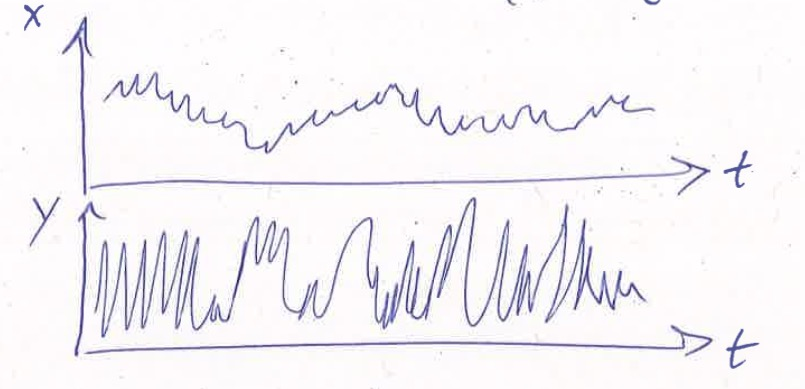
\includegraphics[width=0.75\linewidth]{images/Screenshot 2024-05-21 at 18.18.51.jpg}
\end{figure}

VAR of order 1 is a model of the form: 
\begin{align*}
    y_t&= \alpha+\rho y_{t-1} + \theta x_{t-1} + \varepsilon_t\\
    x_t&= \beta + \xi y_{t-1} + \zeta x_{t-1} + u_t
\end{align*}
Can be written in matrix notation, helpful for more than 2 time series\\

\noindent
Consider $(X_{t,1}, X_{t,2})$ as a bivariate time series. \\
$(X_{t,1}, X_{t,2},\cdots,X_{t,\kappa})$ as a $\kappa$-variate time series. \\

\noindent
Call the vector of observations at time $t$: $X_t$ \\
Similar for $\varepsilon_t$ \\
Then $VAR(1)$ model is written \[
    x_t= \Phi X_{t-1} + \varepsilon_t
\] \quad where $\Phi$ is a matrix

\noindent
\rule{\linewidth}{0.4pt}
\begin{align*}
    \text{If } &y_t = x_{t,1}  \quad x_t = x_{t,2} \ ,\  \Phi = \begin{pmatrix}
\rho & \theta \\
\xi & \zeta 
\end{pmatrix} \\
&\varepsilon_t = \varepsilon_{t,1}  \quad u_t = \varepsilon_{t,2} \\
\text{Then} \\
x_t&= \Phi x_{t-1}+ \varepsilon_t \Leftrightarrow \begin{matrix}
    y_t=\rho y_{t-1} + \theta x_{t-1} + \varepsilon \\
    x_t = \xi y_{t-1} + \zeta x_{t-1} + u_t
\end{matrix}
\end{align*}

Multivariate time series with notation: $X_t = \Phi X_{t-1}  +\varepsilon_t$
\begin{itemize}
    \item Can estimate $\hat{\Phi}$ with maximal likelihood
    \item IRFs - Still problems in defining them
    \begin{itemize}
        \item There are several
        \item For univariate time series we used a MA($\infty$) representation
        \item Will have to take a stand on whether $\varepsilon_{t,1}$ or $\varepsilon_{t,2}$ comes first
        \item There are other alternatives (long run restrictions, ...) 
    \end{itemize}
\end{itemize}
\[
X_t = \Phi X_{t-1} + \varepsilon_t \quad \quad X_t = \begin{pmatrix}
    X_{t,1} \\
    X_{t,2}
\end{pmatrix} ,\ \varepsilon_t = \begin{pmatrix}
    \varepsilon_{t,1}\\
    \varepsilon_{t,2}
\end{pmatrix}
\]
Several impulse response functions:
\begin{align*}
    & \frac{\partial x_{t+r, 1}}{\partial \varepsilon_{t, 1}} & \quad \frac{\partial x_{t+r, 2}}{\partial \varepsilon_{t, 1}} \\
    & \frac{\partial x_{t+r, 1}}{\partial \varepsilon_{t, 2}} & \quad \frac{\partial x_{t+r, 2}}{\partial \varepsilon_{t, 2}}
\end{align*}

\noindent
\rule{\linewidth}{0.4pt}
\noindent
What is a MA($\infty$) for a VAR?\\
Want this to facilitate calculating above 4 listed derivatives.

\begin{align*}
    & \text{Let } B X_t = X_{t-1} \text{ again.} \\
    & B = \begin{pmatrix}
    B_{1-\text{dim}} & 0 \\
    0 & B_{1-\text{dim}}
    \end{pmatrix}
\end{align*}

\[
B \begin{pmatrix}
x_{t,1} \\
x_{t,2}
\end{pmatrix}
= \begin{pmatrix}
B_{1-\text{dim}} x_{t,1} \\
B_{1-\text{dim}} x_{t,2}
\end{pmatrix}
= \begin{pmatrix}
x_{t-1,1} \\
x_{t-1,2}
\end{pmatrix}
\]

\[
(I - \Phi B) x_t = \varepsilon_t
\]

Form \((I - \Phi B)^{-1} \varepsilon_t = X_t\):

\[
X_t = I \varepsilon_t + \Phi B \varepsilon_t + (\Phi B)^2 \varepsilon_t + (\Phi B)^3 \varepsilon_t + \cdots
\]

\subsubsection{Structural VAR}
\begin{itemize}
    \item A class of Models for Multivariate Time Series 
\end{itemize}

Think about a 2-variate time series: 
\begin{align*}
    Y_{1t} &= a_1 + b_1y_{2t} + \psi_{11} Y_{1t-1} + \psi_{12} Y_{2t-1} + \varepsilon_{1t} \\
    Y_{2t} &=  a_1 + b_2 y_{1t} + \psi_{21} Y_{1t-1} + \psi_{22} Y_{2t-1} + \varepsilon_{2t}
\end{align*}
What is different here, relative to all previous time series models we saw?\\

Contemporaneous $Y$s can be seen on the right hand side (e.g., $\dots +b_1 Y_{2t}+ \cdots$ note that the '$t$' instead of '$t-1$')\\

This is like a system of equations changing over time.  
\begin{align*}
    \text{Let } Z_{1t} &= \psi_{11}Y_{1t-1}+\psi_{12}Y_{2t-1} +\varepsilon_{1t} + a_1 \\
    Z_{2t} &= \psi_{21} Y_{1t-1} + \psi_{22} Y_{2t-1} + \varepsilon_{2t} + a_2
\end{align*}
\textcolor{red}{ REST !!!}\\

Solve a system to get $Y_{1t}, Y_{2t} $
\textcolor{red}{GRAPH} \\

\fbox{$\Rightarrow$ This is like a Model of a moving equilibrium. (moving over $t$)} \\

How to proceed: \\

Corresponding Reduced Form VAR is:
\begin{align*}
    Y_{1t} &= \mu_1 + \xi_{11} + Y_{1t-1} + \xi_{12} Y_{2t-1} + U_{1t}\\
    Y_{2t} &= \mu_2 + \xi_{21} Y_{1t-1} + \xi_{22} Y_{2t-1} + U_{2t}
\end{align*}
This is a VAR model with changed letters 
\begin{itemize}
    \item no contemporaneous $Y_{1t}$ or $Y_{2t}$ on the right hand side
    \item Coefficients are different
    \item Residuals are $U_{1t}$ and $U_{2t}$ now
\end{itemize}
How does the reduced form relate to the structural model? 
\begin{align*}
    \text{Let } Y_t = \begin{pmatrix}
        Y_{1t} \\
        Y_{2t}
    \end{pmatrix},\ U_t = \begin{pmatrix}
        U_{1t} \\
        U_{2t}
    \end{pmatrix},\  \varepsilon_t = \begin{pmatrix}
        \varepsilon_{1t}\\
        \varepsilon_{2t}
    \end{pmatrix} \ etc.
\end{align*}

\underline{Structural Model}
\begin{align*}
    Y_t = a + B_{Y_t} + \psi_{Y_{t-1}} + \varepsilon_t \quad \text{where } B=\begin{pmatrix}
        0 & b_1  
    \end{pmatrix}
\end{align*}
\textcolor{red}{RESST}\\

Can relate the two models by inverting $I-B$ like follows:\\

Note: in Structural Model \begin{align*}
    (I-B)_{Y_t} &= a + \psi_{Y_{t-1}} + \varepsilon_t \\
    \Rightarrow Y_t &= (I-B)^{-1} a + (I-B)^{-1} \psi_{Y_{t-1}}+ (I-B)^{-1}\varepsilon_t \\
    \text{plug in Reduced Form} \\
    Y_t&= \mu+ \xi_{Y_{t-1}}+ U_t \\
    \Rightarrow \mu&= (I-B)^{-1}a,\ \xi= (I-B)^{-1} \psi_{Y_{t-1}} \\
    \mu &= (I-B)^{-1} \varepsilon_t
\end{align*}

$\Rightarrow$ Can go back and forth via this dictionary. \underline{With 1 exception!}\\


In structural model: 
\begin{align*}
    Y_{1t} &= a_1 + b_1 Y_{2t} + \cdots + \varepsilon_{1t} \\
    Y_{2t} &= a_2 + b_2 Y_{1t} + \cdots + \varepsilon_{2t}
\end{align*}
The entire purpose is to evaluate independent shocks to $\varepsilon_{1t}$ and $\varepsilon_{2t}$ \\
So \underline{structure} is that $\varepsilon_{1t} \perp \varepsilon_{2t}$ (Shocks are assumed independent) \[
Cov(\varepsilon_{1t}, \varepsilon_{2t}) = 0
\]
Problem: in Reduced Form model, \[
Cov(U_{1t}, U_{2t}) \neq 0
\]
So reduced form and structural models have different number of parameters. \\

Need to make further assumptions on how $U_t$ relate to $\varepsilon_t$ to make progress on impulse responses or just estimating $\psi,a$. \\

\noindent
\underline{Many options:}
\begin{itemize}
    \item Option 1: Take a stand on which ($\varepsilon_{1t}$ or $\varepsilon_{2t}$) is first in the following way:
    \begin{itemize}
        \item If $\varepsilon_{1t}$ is first, then $\varepsilon_{2t}$ does not directly hit $Y_{1t}$ (Order shocks and exclude $b_1$)
        \item[] $Y_{1t} = a_1 + 0\cdot Y_{2t} + \cdots + \varepsilon_{1t}$
        \item[] $Y_{2t} = a_2 + b_2 \cdot Y_{1t} + \cdots + \varepsilon_{2t}$
        \begin{itemize}
            \item Can now do recursion (because we set $b_1=0$)
            \item If Shock $\varepsilon_{1t}$, understand directly what happens to $Y_{1t}$. Then can more easily think what happens from subsequent $\varepsilon_{2t}$ shock.
        \end{itemize}
    \end{itemize}
\end{itemize}

\noindent
\underline{Example:} \quad Currencies \\
with bivariate USD + CHF value (versus some numerair, in case you decide against USD) \\
Shocks to USD will immediately affect CHF. But shocks to CHF might take time to hit USD. \\

Have to order the shocks to identify IRFs (in option 1). \\

Note: How many params: 
\begin{itemize}
    \item In structural 9 total with $b_1=0$ and $Cov(\varepsilon_{1t}, \varepsilon_{2t})=0$ restrictions
    \item In reduced form: also 9 total model
\end{itemize}
$\Rightarrow$ Same amount of info in structural and reduced form 

\begin{itemize}
    \item Option 2: Long run restrictions. 
    \begin{itemize}
        \item Model: $\begin{pmatrix}
            \Delta Y_t \\
            U_t
        \end{pmatrix}$ is stationary + shocks one $\begin{pmatrix}
            e_d \\
            e_s
        \end{pmatrix}$
        \begin{itemize}
            \item $s_0: e_d \perp e_s$ and $e_d$ shocks $\Delta Y_t$, $e_s$ shocks $U_t$
        \end{itemize}
        \item Restriction: In the long run, $e_d$ has no effect on $Y_t$ itself (not differenced) 
    \end{itemize}
\end{itemize}

Blanchard + Quad 1986: 
\begin{itemize}
    \item Model $\begin{pmatrix}
        \Delta Y_t \\
        U_t
    \end{pmatrix}$
    \begin{itemize}
        \item where $Y_t$ is output GNP
        \item where $U_t$ is unemployment
    \end{itemize}
    \item In MA representation: 
    \begin{align*}
        \begin{pmatrix}
            \Delta Y_t \\
            U_t
        \end{pmatrix} &= \Theta_0 \begin{pmatrix}
            e_{d_t} \\
            e_{s_t}
        \end{pmatrix} + \Theta_1 \begin{pmatrix}
            e_{d_{t-1}} \\
            e_{s_{t-1}}
        \end{pmatrix} + \Theta_2 \begin{pmatrix}
            e_{d_{t-2}}\\
            e_{s_{t-2}}
        \end{pmatrix} + \cdots \\
        \text{Then } &\sum_{i=1}^\infty \left[ \Theta_i \right]_{11} = 0_0 \Rightarrow \text{Identification too}
    \end{align*}
\end{itemize}

\fbox{Key Point: Cannot estimate a structural VAR without at least one economic assumption!}

\newpage
\section{Time Series Analysis in R}


This is example code from excercise 1: 

\begin{lstlisting}
# time plot of U.S. GNP and various fitted trends
par(mfrow=c(2,2))
par(oma=c(0,2,4,2))

# global quadratic trend
plot(x=1947.25+gnp.t,y=gnp.v,type="b",ylim=c(200,800),xlab="time",ylab="U.S. GNP",main="Global quadratic trend",col="green4")
lines(1947.25+gnp.t,predict(object=gqt.lm),col="blue")
legend(x="topleft",legend=c("actual values","estimated global trend"),col=c("green4","blue","red"),lty=c(1,1),pch=c(1,-1))

# global cubic trend
plot(x=1947.25+gnp.t,y=gnp.v,type="b",ylim=c(200,800),xlab="time",ylab="U.S. GNP",main="Global cubic trend",col="green4")
lines(1947.25+gnp.t,predict(object=gct.lm),col="blue")

# global multiplicative exponential trend
plot(x=1947.25+gnp.t,y=gnp.v,type="b",ylim=c(200,800),xlab="time",ylab="U.S. GNP",main="Global multiplicative exponential trend",col="green4")
lines(1947.25+gnp.t,exp(predict(object=gmet.lm)),col="blue")

# global additive exponential trend
plot(x=1947.25+gnp.t,y=gnp.v,type="b",ylim=c(200,800),xlab="time",ylab="U.S. GNP",main="Global additive exponential trend",col="green4")
lines(1947.25+gnp.t,predict(object=gaet.nls),col="blue")

mtext(text="Time plots of U.S. GNP and fitted trends",side=3,line=0,outer=T)
\end{lstlisting}

\begin{figure}[ht]
\centering
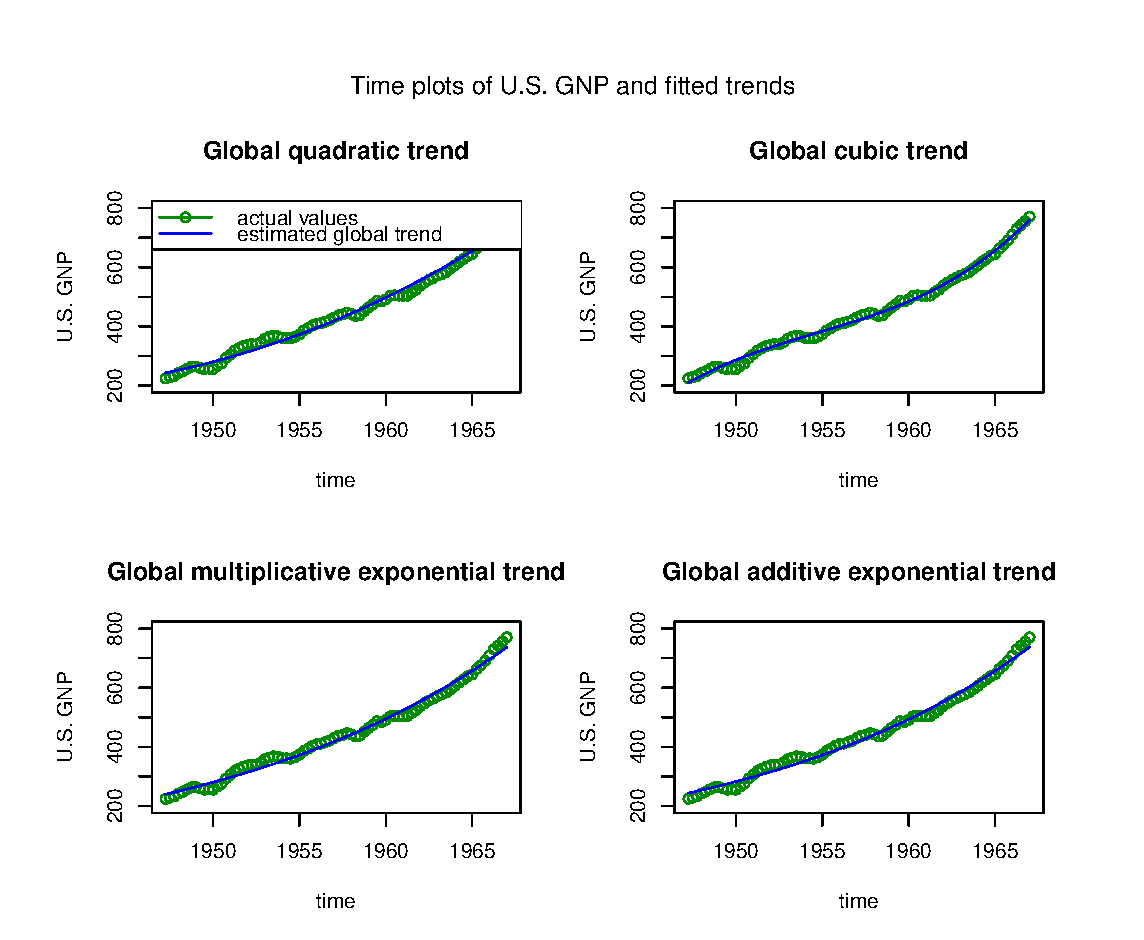
\includegraphics[width=0.8\textwidth]{plots/Rplot1.pdf}
\caption{various fits}
\end{figure}

\newpage
\section{Appendix: Mathematical Reminders}
\subsection{Arithmetic Series}
General Formula: \[
S_n=\frac{n(a_1 + a_n)}{2}
\]

\subsection{Geometric Series}
Given an integer $n_0$ and a real number $0<a \neq 1$:
\begin{align*}
    \sum_{i=0}^n a^{i} = 1 + a + a^2 + \cdots +a^n = \frac{1-a^{n+1}}{1-a} \label{GEOSeries}
\end{align*}
Given an integer $n_0$ and a real number $|a|<1$:
\begin{align*}
    \sum_{i=0}^\infty a^{i} = \frac{1}{1-a}
\end{align*}

\subsection{Determinant Calculation} \label{Determinant Calculation }

Calculating the determinant of a matrix is a fundamental concept in linear algebra. The determinant is a scalar value that can be computed from the elements of a square matrix and provides important properties about the matrix, such as whether it is invertible.

\subsection*{Steps to Calculate the Determinant}

\subsubsection*{Determinant of a 2x2 Matrix}
For a $2 \times 2$ matrix:
\[
A = \begin{pmatrix}
a & b \\
c & d
\end{pmatrix}
\]
The determinant, denoted as $\det(A)$ or $|A|$, is calculated as:
\[
\det(A) = ad - bc
\]

\subsubsection*{Determinant of a 3x3 Matrix}
For a $3 \times 3$ matrix:
\[
A = \begin{pmatrix}
a & b & c \\
d & e & f \\
g & h & i
\end{pmatrix}
\]
The determinant is calculated using the rule of Sarrus or cofactor expansion:
\[
\det(A) = a(ei - fh) - b(di - fg) + c(dh - eg)
\]

\subsubsection*{General Case for $n \times n$ Matrix}
For larger matrices, the determinant can be calculated by cofactor expansion along any row or column. The process involves breaking the determinant into smaller determinants of submatrices.


\subsection{Maximum Likelihood Estimation (MLE)}

Maximum Likelihood Estimation (MLE) is a method for estimating the parameters of a statistical model. The main idea is to find the parameter values that maximize the likelihood function, which measures how well the model explains the observed data.

\subsubsection*{Steps in Maximum Likelihood Estimation}

1. \textbf{Define the Likelihood Function}:
   Given a set of observations \(\{x_1, x_2, \ldots, x_n\}\), and a statistical model with parameters \(\theta\), the likelihood function \(L(\theta)\) is defined as the probability of observing the given data under the model:
   \[
   L(\theta) = P(X_1 = x_1, X_2 = x_2, \ldots, X_n = x_n \mid \theta)
   \]
   For independent observations, the likelihood function can be written as:
   \[
   L(\theta) = \prod_{i=1}^n P(X_i = x_i \mid \theta)
   \]

2. \textbf{Log-Likelihood Function}:
   It is often more convenient to work with the log-likelihood function, which is the natural logarithm of the likelihood function. The log-likelihood function \(\ell(\theta)\) is given by:
   \[
   \ell(\theta) = \log L(\theta) = \sum_{i=1}^n \log P(X_i = x_i \mid \theta)
   \]

3. \textbf{Maximize the Log-Likelihood}:
   Find the parameter values \(\hat{\theta}\) that maximize the log-likelihood function. This involves solving the following optimization problem:
   \[
   \hat{\theta} = \arg\max_\theta \ell(\theta)
   \]
   This can be done using calculus by setting the derivative of the log-likelihood function with respect to \(\theta\) to zero and solving for \(\theta\):
   \[
   \frac{\partial \ell(\theta)}{\partial \theta} = 0
   \]

4. \textbf{Second Derivative Test}:
   To ensure that the solution obtained is a maximum, the second derivative of the log-likelihood function can be evaluated. If the second derivative is negative, it indicates a maximum:
   \[
   \frac{\partial^2 \ell(\theta)}{\partial \theta^2} < 0
   \]

\subsubsection*{General Log-Likelihood Formula Using Residuals}

For models with normally distributed residuals, the general log-likelihood function can be expressed as:

\[ \ell(\theta) \propto -\sum_{t=1}^{T} \left( \log(\sigma_t) + \frac{1}{2} \frac{\text{residual}_t^2}{\sigma_t^2} \right) \]

where:
- \(\theta\) represents the parameter vector (e.g., \(\mu, \phi, \theta, \alpha, \beta\)).
- \(\sigma_t^2\) is the conditional variance (which can be constant or time-varying).
- \(\text{residual}_t\) represents the residuals specific to the model.

\subsubsection*{Example: Normal Distribution}

Consider a simple example where we assume the data \(\{x_1, x_2, \ldots, x_n\}\) are drawn from a normal distribution with unknown mean \(\mu\) and known variance \(\sigma^2\).

1. \textbf{Likelihood Function}:
   \[
   L(\mu) = \prod_{i=1}^n \frac{1}{\sqrt{2\pi\sigma^2}} \exp\left(-\frac{(x_i - \mu)^2}{2\sigma^2}\right)
   \]

2. \textbf{Log-Likelihood Function}:
   \[
   \ell(\mu) = \sum_{i=1}^n \left( -\frac{1}{2} \log(2\pi\sigma^2) - \frac{(x_i - \mu)^2}{2\sigma^2} \right)
   \]

3. \textbf{Maximize the Log-Likelihood}:
   Taking the derivative with respect to \(\mu\) and setting it to zero:
   \[
   \frac{\partial \ell(\mu)}{\partial \mu} = \sum_{i=1}^n \frac{x_i - \mu}{\sigma^2} = 0
   \]
   Solving for \(\mu\):
   \[
   \hat{\mu} = \frac{1}{n} \sum_{i=1}^n x_i
   \]
   This is the sample mean, which is the MLE for the mean of a normal distribution with known variance.

\subsubsection*{Example: ARMA Model}

For an ARMA(p, q) model, the residuals are:

\[ \text{residual}_t = X_t - \mu - \sum_{i=1}^p \phi_i X_{t-i} - \sum_{j=1}^q \theta_j \epsilon_{t-j} \]

The log-likelihood function is:

\[ \ell(\mu, \phi, \theta, \sigma^2) \propto -\sum_{t=1}^{T} \left( \log(\sigma) + \frac{\text{residual}_t^2}{2\sigma^2} \right) \]

\subsubsection*{Example: ARMA-GARCH Model}

For an ARMA(p, q)-GARCH(h, k) model, the residuals are:

\[ \text{residual}_t = X_t - \mu - \sum_{i=1}^p \phi_i X_{t-i} - \sum_{j=1}^q \theta_j \epsilon_{t-j} \]

The conditional variance \(\sigma_t^2\) is time-varying:

\[ \sigma_t^2 = \alpha_0 + \sum_{i=1}^h \alpha_i \epsilon_{t-i}^2 + \sum_{j=1}^k \beta_j \sigma_{t-j}^2 \]

The log-likelihood function is:

\[ \ell(\mu, \phi, \theta, \alpha, \beta) \propto -\sum_{t=1}^{T} \left( \log(\sigma_t) + \frac{\text{residual}_t^2}{\sigma_t^2} \right) \]

\subsubsection*{Advantages and Disadvantages}

\textbf{Advantages}:
\begin{itemize}
    \item Provides a unified framework for parameter estimation.
    \item Asymptotically efficient: MLE estimators achieve the lowest possible variance among unbiased estimators for large sample sizes.
\end{itemize}

\textbf{Disadvantages}:
\begin{itemize}
    \item Requires the specification of the likelihood function, which might be complex for some models.
    \item Can be computationally intensive, especially for large datasets or complex models.
    \item Sensitive to model assumptions; incorrect assumptions can lead to biased estimates.
\end{itemize}






\end{document}
